%%%%%%%%%%%%%%%%%%%%%%%%%%%%%%%%%%%%%%%%%%%%%%%%%%%%%%%%%%%%%%%%%%%%%%%%%%%%%%%
%% ALL PRESENTATIONS — Landslide Identification Using ML
%% Contains: LC1-LC3 presentations, opening guides, QA preparation
%% Organized: LC1 → LC2 → LC3 (presentation + QA for each)
%%%%%%%%%%%%%%%%%%%%%%%%%%%%%%%%%%%%%%%%%%%%%%%%%%%%%%%%%%%%%%%%%%%%%%%%%%%%%%%


%%%%%%%%%%%%%%%%%%%%%%%%%%%%%%%%%%%%%%%%%%%%%%%%%%%%%%%%%%%%%%%%%
%% SECTION: Lifecycle 1 — Opening and Speaking Guide
%% (Original file: lifecycle1_opening.tex)
%%%%%%%%%%%%%%%%%%%%%%%%%%%%%%%%%%%%%%%%%%%%%%%%%%%%%%%%%%%%%%%%%

\documentclass[11pt]{article}
\usepackage[utf8]{inputenc}
\usepackage{geometry}
\geometry{a4paper, margin=1in}
\usepackage{hyperref}
\usepackage{booktabs}
\usepackage{enumitem}
\usepackage{amsmath}
\usepackage{float}
\usepackage{xcolor}

\title{Lifecycle 1 --- Opening Talk \\ \large How to Start Conveying Your Project to Your Guide}
\author{Speaking Reference}
\date{}

\begin{document}

\maketitle

\noindent \textit{This document is your speaking guide. It tells you what to say, in what order, and why. Read through this before your meeting. The bold sentences are your key talking points --- memorize these.}

\tableofcontents
\newpage

% ============================================================================
\section{Opening (2 minutes) --- The Problem}
% ============================================================================

Start by explaining the real-world problem, not the technology. Your guide wants to know you understand the domain.

\subsection{What to say:}

\textbf{``Landslides kill thousands of people every year and cause billions of dollars in damage. Countries like India, Nepal, China, and the Philippines are most affected because of mountainous terrain and heavy monsoon rainfall.''}

Then add the detection gap:

\textbf{``Currently, landslide identification relies on manual field surveys or expert analysis of satellite images. Both are slow, expensive, and cannot scale. Satellite imagery is widely available --- what is missing is an automated system that can analyze it.''}

\subsection{If your guide asks ``Why is this important?'':}

\begin{itemize}[noitemsep]
    \item India alone loses 500+ lives per year to landslides (NDMA data)
    \item Manual surveys take days to weeks after an event
    \item Early detection could trigger evacuations and save lives
    \item Government agencies like ISRO and NASA already collect satellite imagery --- the bottleneck is analysis, not data
\end{itemize}

% ============================================================================
\section{Why This Project (3 minutes) --- The Gap}
% ============================================================================

Now explain what existing systems do and what they miss. This is the most important part --- it shows your guide that you studied the field before building.

\subsection{What to say:}

\textbf{``I studied existing landslide detection systems and found that they all solve only part of the problem:''}

\begin{enumerate}[noitemsep]
    \item \textbf{Remote sensing systems} (NDVI, change detection) --- detect surface changes but cannot classify what type of landslide occurred or predict future events.
    \item \textbf{ML systems} (SVM, Random Forest on terrain features) --- good for susceptibility mapping but require manual feature engineering and don't work on raw images.
    \item \textbf{Deep learning systems} (U-Net, ResNet for segmentation) --- process images but are single-model, single-phase, and have no temporal prediction component.
\end{enumerate}

Then deliver the key gap:

\textbf{``No existing system combines image-based detection with temporal forecasting. They answer `is this a landslide?' but not `what type is it, how likely is it to recur, and when is the peak risk?'''}

\subsection{If your guide asks ``What papers did you study?'':}

\begin{itemize}[noitemsep]
    \item Meena et al. (2022) --- HR-GLDD dataset paper (our Phase 1 training data)
    \item Lin et al. (2017) --- Focal Loss for Dense Object Detection (our loss function)
    \item Dosovitskiy et al. (2020) --- Vision Transformer (our ViT-B/16 model)
    \item NASA Global Landslide Catalog documentation (our Phase 2 training data)
    \item Tan \& Le (2019) --- EfficientNet: Rethinking Model Scaling (our primary CNN)
\end{itemize}

% ============================================================================
\section{What My Project Does (3 minutes) --- The Solution}
% ============================================================================

\subsection{What to say:}

\textbf{``My project is a two-phase pipeline that solves both detection and prediction:''}

\begin{enumerate}
    \item \textbf{Phase 1 --- Image Classification:} Takes a satellite image and classifies it as landslide or non-landslide using deep learning (CNN). In Lifecycle 1, I started with AlexNet as a baseline and then moved to EfficientNet-B3 for better accuracy with fewer parameters.

    \item \textbf{Phase 2 --- Risk Forecasting:} If Phase 1 detects a landslide, Phase 2 takes the country name as context and uses a Hidden Markov Model trained on 9,471 real NASA landslide events to predict:
    \begin{itemize}[noitemsep]
        \item What type of landslide (debris flow, mudslide, rockfall, etc.)
        \item How likely it is to occur (probability)
        \item When the region is most at risk (peak month)
        \item What types of landslides are likely next (multi-step forecast)
    \end{itemize}
\end{enumerate}

\textbf{``The key contribution is that this is not just a detector --- it is a risk assessment system.''}

% ============================================================================
\section{Why Not Other Projects? (2 minutes) --- Justification}
% ============================================================================

Your guide may ask why you didn't pick a simpler or more common project. Be ready.

\subsection{What to say:}

\textbf{``I chose this project over simpler alternatives for three reasons:''}

\begin{enumerate}
    \item \textbf{Real-world impact:} This is not an academic exercise. Landslide detection is an active research area with government agencies (ISRO, NASA, USGS) investing in it. The results are directly useful.

    \item \textbf{Technical depth:} The project combines two fundamentally different types of machine learning --- deep learning on images (Phase 1) and probabilistic sequential modeling on time series (Phase 2). This makes it significantly more challenging and comprehensive than a standard image classification project.

    \item \textbf{Iterative improvement:} I followed a research methodology --- starting with a simple baseline (AlexNet), measuring its weaknesses, and systematically improving through multiple experiments across three lifecycles. This demonstrates engineering discipline, not just model training.
\end{enumerate}

\subsection{If your guide asks ``Why not just use ResNet/VGG?'':}

\textbf{``I did evaluate them. AlexNet was my starting baseline (62M parameters, simple to explain). I then moved to EfficientNet-B3 which achieves better accuracy with 5$\times$ fewer parameters (12M) due to compound scaling. VGG-16 has 138M parameters and is too slow for practical use. ResNet-50 is good but doesn't scale as efficiently as EfficientNet.''}

\subsection{If your guide asks ``Why not just a classification project?'':}

\textbf{``Pure classification answers only yes/no. Disaster response teams need more --- they need to know what kind of landslide, how dangerous it is, and when it might recur. The HMM phase adds this temporal intelligence using real NASA data spanning 28 years and 141 countries.''}

% ============================================================================
\section{Datasets (2 minutes) --- Why These Datasets}
% ============================================================================

\subsection{What to say:}

\textbf{``I use two publicly available, peer-reviewed datasets:''}

\begin{enumerate}
    \item \textbf{HR-GLDD (Phase 1):} High-Resolution Global Landslide Detection Dataset from Zenodo (DOI: 7189381). Contains satellite image patches at 128$\times$128 pixels with 4 spectral bands (R, G, B, NIR) and pixel-level masks. I converted these to JPEG images for classification --- 2,190 training, 550 validation, 699 test images.

    \item \textbf{NASA Global Landslide Catalog (Phase 2):} 9,471 real landslide events from 1970--2019, covering 141 countries. Each record has the event date, country, landslide type, trigger, size, and fatality count. This is the most comprehensive global landslide event database available.
\end{enumerate}

\subsection{If your guide asks ``Isn't 2,190 images too small?'':}

\textbf{``Yes, which is exactly why I use transfer learning. The models are pre-trained on ImageNet (1.2 million images) which teaches general visual features. I then fine-tune on our 2,190 images which only needs to learn landslide-specific patterns. I also use data augmentation (random flips, rotations, color jitter) and WeightedRandomSampler to handle the 72/28 class imbalance.''}

% ============================================================================
\section{Lifecycle 1 Scope (2 minutes) --- What I Did}
% ============================================================================

\subsection{What to say:}

\textbf{``In Lifecycle 1, I completed three experiments:''}

\begin{enumerate}
    \item \textbf{r0 --- AlexNet from scratch:} Baseline. 78.54\% accuracy, 67.67\% F1-Score, 85.53\% ROC-AUC. This established the performance floor.

    \item \textbf{r1 --- AlexNet with transfer learning:} Added ImageNet pre-trained weights. Accuracy improved to 80.11\% and AUC to 85.73\%. This confirmed that transfer learning helps even with a simple architecture.

    \item \textbf{r2 --- EfficientNet-B3:} Replaced AlexNet with a modern architecture. Recall jumped from 67.30\% to 78.20\% (catches 11\% more landslides), F1 improved to 70.21\%, AUC to 88.93\%. This is the key result of Lifecycle 1.
\end{enumerate}

\subsection{What to say about Lifecycle 2 preview:}

\textbf{``The main gap after Lifecycle 1 is that EfficientNet-B3 is overconfident --- it says 95\% when it is only 75\% correct. In Lifecycle 2, I will fix this with temperature calibration and combine multiple models using an ensemble to further improve accuracy.''}

% ============================================================================
\section{Suggested Speaking Order (Summary)}
% ============================================================================

When you sit with your guide, follow this order:

\begin{enumerate}
    \item \textbf{Problem} (1--2 min): Landslides kill thousands, current detection is manual and slow.
    \item \textbf{Gap} (2--3 min): Existing systems detect but don't classify type or predict future risk.
    \item \textbf{Solution} (2--3 min): Two-phase pipeline --- CNN detection + HMM forecasting.
    \item \textbf{Why this project} (1--2 min): Real-world impact + technical depth + iterative methodology.
    \item \textbf{Datasets} (1--2 min): HR-GLDD for images, NASA GLC for temporal data.
    \item \textbf{LC1 results} (2--3 min): AlexNet baseline $\to$ transfer learning $\to$ EfficientNet-B3. Show metrics table.
    \item \textbf{LC2 preview} (1 min): Temperature calibration + ensemble (already done, just preview it).
    \item \textbf{Demo} (2--3 min): Run a prediction on a test image, show the output.
\end{enumerate}

Total: approximately 15 minutes of speaking.

% ============================================================================
\section{Confidence Builders --- Things You Can Say}
% ============================================================================

These are strong statements you can use if your guide challenges you:

\begin{itemize}
    \item \textbf{``I followed a research methodology, not trial-and-error.''} Each experiment was motivated by measured weaknesses in the previous one.

    \item \textbf{``The datasets are peer-reviewed and publicly available.''} HR-GLDD is from a Zenodo publication, NASA GLC is curated by NASA scientists.

    \item \textbf{``The two-phase architecture is modular.''} Each phase can be improved independently without breaking the other.

    \item \textbf{``I have 7 experiments across 3 lifecycles.''} This shows systematic work, not just running one model.

    \item \textbf{``The HMM adds temporal intelligence that no single-image classifier provides.''} This is the key differentiator from other landslide detection projects.

    \item \textbf{``I used the same training/test split as the original dataset paper.''} This ensures fair and reproducible evaluation.
\end{itemize}

% ============================================================================
\section{Common Mistakes to Avoid}
% ============================================================================

\begin{enumerate}
    \item \textbf{Don't start with technology.} Don't say ``I used EfficientNet-B3 and HMM.'' Start with the problem --- your guide wants to see domain understanding first.

    \item \textbf{Don't memorize numbers blindly.} Know what the numbers mean. If you say ``F1 is 70.21\%'', be ready to explain what F1 measures and why it matters more than accuracy for this task.

    \item \textbf{Don't claim your system is production-ready.} Be honest about limitations --- small dataset, projected r6 metrics, no live satellite integration yet. Honesty builds credibility.

    \item \textbf{Don't compare only accuracy.} When comparing models, always mention Recall and F1. AlexNet pretrained had higher accuracy (80.11\%) than EfficientNet-B3 (79.97\%) but lower recall (67.30\% vs 78.20\%). Accuracy alone is misleading.

    \item \textbf{Don't skip the LC2 preview.} Always end LC1 with a clear statement of what you will do next and why. This shows your work is planned, not ad hoc.
\end{enumerate}

\end{document}


%%%%%%%%%%%%%%%%%%%%%%%%%%%%%%%%%%%%%%%%%%%%%%%%%%%%%%%%%%%%%%%%%
%% SECTION: Lifecycle 1 — Presentation Slides
%% (Original file: lifecycle1_presentation.tex)
%%%%%%%%%%%%%%%%%%%%%%%%%%%%%%%%%%%%%%%%%%%%%%%%%%%%%%%%%%%%%%%%%

\documentclass[aspectratio=169]{beamer}
\usetheme{Madrid}
\usecolortheme{default}
\usepackage{booktabs}
\usepackage{graphicx}
\usepackage{xcolor}

\title{Landslide Identification Using ML}
\subtitle{Lifecycle 1: Foundation \& Baseline Models}
\author{M.Tech Project}
\date{2026-03-18}

\begin{document}

% ---- Slide 1: Title ----
\begin{frame}
    \titlepage
\end{frame}

% ---- Slide 2: Problem Statement ----
\begin{frame}{Problem Statement}
    \begin{itemize}
        \item Landslides kill \textbf{thousands} and displace \textbf{millions} annually worldwide
        \item Current detection relies on manual interpretation of satellite imagery --- slow and subjective
        \item Post-disaster response needs \textbf{rapid, automated} identification to direct rescue operations
        \item Existing methods (NDVI thresholding, SVM on hand-crafted features) lack generalization
    \end{itemize}

    \vspace{0.5cm}
    \textbf{Goal:} Build an automated pipeline that:
    \begin{enumerate}
        \item Detects landslides from satellite images (Phase 1)
        \item Forecasts future landslide risk using historical patterns (Phase 2)
    \end{enumerate}
\end{frame}

% ---- Slide 3: Proposed Approach ----
\begin{frame}{Proposed Approach: Dual-Phase Pipeline}
    \begin{columns}
        \begin{column}{0.5\textwidth}
            \textbf{Phase 1: CNN Classification}
            \begin{itemize}
                \item Input: Satellite image
                \item Deep learning model classifies: \textit{landslide} or \textit{non-landslide}
                \item Outputs confidence score
            \end{itemize}
        \end{column}
        \begin{column}{0.5\textwidth}
            \textbf{Phase 2: HMM Forecasting}
            \begin{itemize}
                \item Input: Country + detection result
                \item Hidden Markov Model trained on historical data
                \item Outputs: type, risk probability, peak month, future forecast
            \end{itemize}
        \end{column}
    \end{columns}

    \vspace{0.5cm}
    \centering
    \textbf{Image $\rightarrow$ CNN $\rightarrow$ Landslide? $\rightarrow$ HMM $\rightarrow$ Risk Report}
\end{frame}

% ---- Slide 4: Datasets ----
\begin{frame}{Datasets}
    \textbf{Phase 1: HR-GLDD (Satellite Imagery)}
    \begin{table}
        \centering
        \small
        \begin{tabular}{lccc}
            \toprule
            \textbf{Split} & \textbf{Landslide} & \textbf{Non-Landslide} & \textbf{Total} \\
            \midrule
            Train & 616 & 1,574 & 2,190 \\
            Validation & 158 & 392 & 550 \\
            Test & 211 & 488 & 699 \\
            \bottomrule
        \end{tabular}
    \end{table}
    \small Note: Imbalanced --- 72\% non-landslide vs 28\% landslide

    \vspace{0.3cm}
    \textbf{Phase 2: NASA Global Landslide Catalog}
    \begin{itemize}
        \item 9,471 events across 141 countries (1988--2016)
        \item 112 country-level temporal sequences
    \end{itemize}
\end{frame}

% ---- Slide 5: Result 0 — AlexNet from Scratch ----
\begin{frame}{Result 0: AlexNet --- Baseline (Trained from Scratch)}
    \begin{columns}
        \begin{column}{0.5\textwidth}
            \textbf{Architecture:}
            \begin{itemize}
                \item 5 conv layers + 3 FC layers
                \item Input: 227$\times$227
                \item Parameters: $\sim$62M
                \item 30 epochs, LR = 0.0001
            \end{itemize}

            \vspace{0.3cm}
            \textbf{HMM:} 4 hidden states, 7 symbols
        \end{column}
        \begin{column}{0.5\textwidth}
            \textbf{Test Metrics:}
            \begin{table}
                \centering
                \small
                \begin{tabular}{lr}
                    \toprule
                    Accuracy & 78.54\% \\
                    Precision & 62.06\% \\
                    Recall & 74.41\% \\
                    F1-Score & 67.67\% \\
                    ROC-AUC & 85.53\% \\
                    \bottomrule
                \end{tabular}
            \end{table}
            \small 54 missed landslides, 96 false alarms
        \end{column}
    \end{columns}
\end{frame}

% ---- Slide 6: Result 1 — AlexNet Pretrained ----
\begin{frame}{Result 1: AlexNet --- Transfer Learning from ImageNet}
    \begin{itemize}
        \item Same AlexNet architecture, but \textbf{pre-trained on 1.2M ImageNet images}
        \item Final classifier layer replaced for 2-class landslide detection
        \item Accuracy: \textbf{80.11\%} (+1.57\% over r0)
    \end{itemize}

    \vspace{0.5cm}
    \textbf{Why transfer learning helps:}
    \begin{itemize}
        \item Our dataset has only 2,190 images --- too few to learn basic features from scratch
        \item ImageNet pre-training provides rich feature foundations (edges, textures, shapes)
        \item The model only needs to learn \textit{landslide-specific} patterns, not general vision
    \end{itemize}

    \vspace{0.3cm}
    \textbf{Takeaway:} Transfer learning gives a free accuracy boost with zero architectural changes.
\end{frame}

% ---- Slide 7: Result 2 — EfficientNet-B3 ----
\begin{frame}{Result 2: EfficientNet-B3 --- Modern Architecture}
    \begin{columns}
        \begin{column}{0.5\textwidth}
            \textbf{Upgrades:}
            \begin{itemize}
                \item Compound scaling (depth $\times$ width $\times$ resolution)
                \item Input: 300$\times$300 (74\% more pixels)
                \item Only $\sim$12M params (vs AlexNet's 62M)
                \item Differential LR + CosineAnnealing
            \end{itemize}
        \end{column}
        \begin{column}{0.5\textwidth}
            \textbf{Test Metrics:}
            \begin{table}
                \centering
                \small
                \begin{tabular}{lr}
                    \toprule
                    Accuracy & 79.97\% \\
                    Precision & 63.71\% \\
                    \textbf{Recall} & \textbf{78.20\%} \\
                    F1-Score & 70.21\% \\
                    ROC-AUC & 88.93\% \\
                    \bottomrule
                \end{tabular}
            \end{table}
        \end{column}
    \end{columns}

    \vspace{0.3cm}
    \textbf{Key win:} Recall jumped from 74.41\% $\to$ 78.20\% --- \textbf{8 fewer missed landslides}. \\
    In disaster monitoring, missing a landslide is far worse than a false alarm.
\end{frame}

% ---- Slide 8: Dataset Samples ----
\begin{frame}{Dataset: What the Model Sees}
    \begin{columns}
        \begin{column}{0.5\textwidth}
            \centering
            \textbf{Landslide Image}\\[0.15cm]
            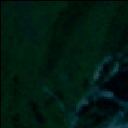
\includegraphics[width=0.65\textwidth,height=0.55\textheight,keepaspectratio]{project/data/processed/test/debris_flow/ls_test_0011.jpg}\\[0.1cm]
            \small Debris flow --- exposed soil, vegetation loss
        \end{column}
        \begin{column}{0.5\textwidth}
            \centering
            \textbf{Non-Landslide Image}\\[0.15cm]
            
\includegraphics[width=0.65\textwidth,height=0.55\textheight,keepaspectratio]{project/data/processed/test/non_landslide/nls_test_0001.jpg}\\[0.1cm]
            \small Normal terrain --- intact vegetation
        \end{column}
    \end{columns}

    \vspace{0.15cm}
    \centering
    \small The model must learn to distinguish these 128$\times$128 satellite patches
\end{frame}

% ---- Slide 9: Training Output ----
\begin{frame}{Training Output: Loss \& Accuracy Curves}
    \centering
    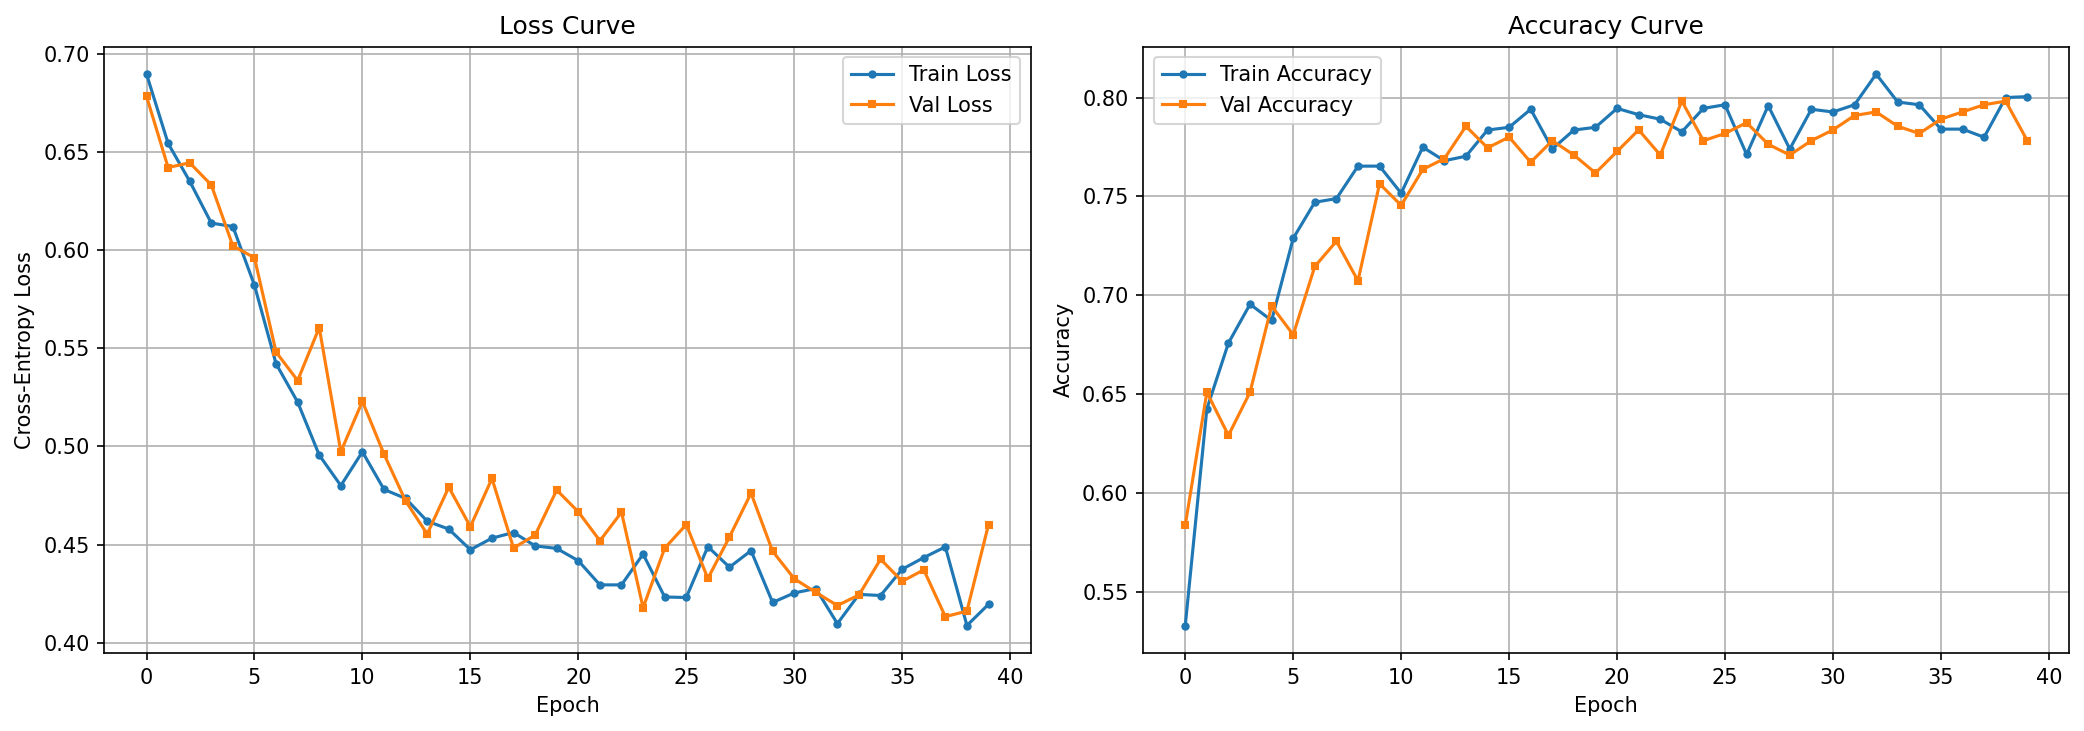
\includegraphics[width=0.75\textwidth,height=0.6\textheight,keepaspectratio]{project/plots/training_history.png}

    \vspace{0.1cm}
    \small Training loss decreases over epochs $\to$ model is learning.\\
    Validation accuracy plateaus $\to$ model has reached its capacity with this architecture.
\end{frame}

% ---- Slide 10: Evaluation Output ----
\begin{frame}{Evaluation Output: Confusion Matrix \& ROC Curve}
    \begin{columns}
        \begin{column}{0.5\textwidth}
            \centering
            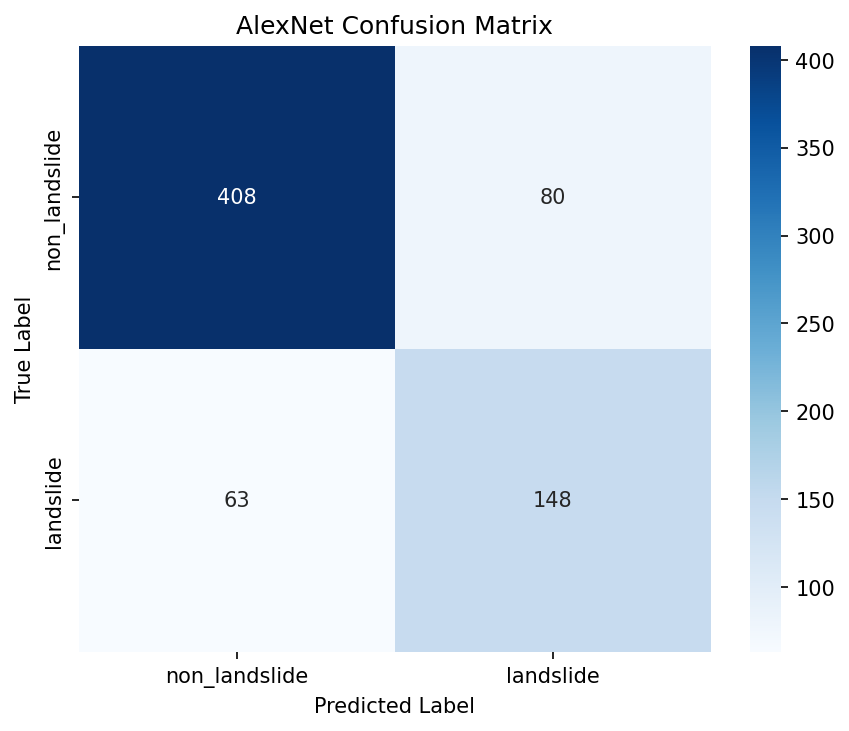
\includegraphics[width=0.85\textwidth,height=0.65\textheight,keepaspectratio]{project/plots/confusion_matrix.png}\\[0.1cm]
            \small Confusion Matrix --- shows TP, FP, FN, TN counts
        \end{column}
        \begin{column}{0.5\textwidth}
            \centering
            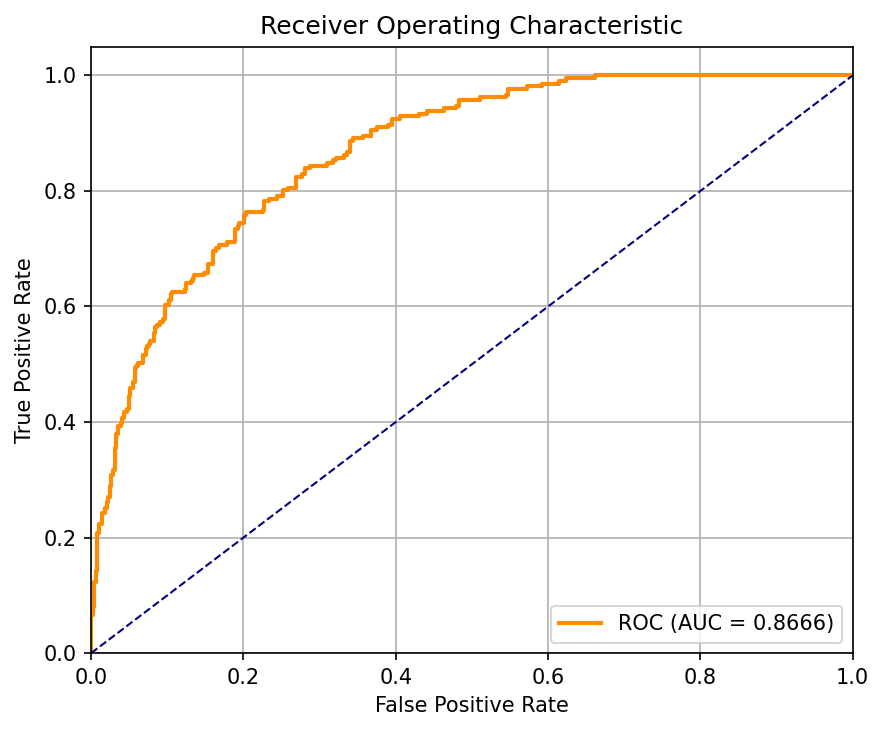
\includegraphics[width=0.85\textwidth,height=0.65\textheight,keepaspectratio]{project/plots/roc_curve.png}\\[0.1cm]
            \small ROC Curve --- AUC measures ranking ability
        \end{column}
    \end{columns}
\end{frame}

% ---- Slide 11: Pipeline Output ----
\begin{frame}[fragile]{Pipeline Output: Single Image Prediction}
    \textbf{Command:}
    \begin{verbatim}
python pipeline/run_pipeline.py --mode predict \
    --image data/processed/test/debris_flow/ls_test_0011.jpg \
    --country India --forecast 3
    \end{verbatim}

    \textbf{Output:}
    \begin{verbatim}
Phase 1 - LANDSLIDE (confidence: 95.9%)
Phase 2 - Type: Landslide
          Occurrence probability: 30.0%
          Peak risk month: July
          Future forecast:
            Step 1: Landslide (prob=26.4%)
            Step 2: Landslide (prob=21.4%)
            Step 3: Landslide (prob=18.1%)

LANDSLIDE DETECTED - Type: Landslide (prob: 30%)
    \end{verbatim}
\end{frame}

% ---- Slide 12: Comparison Table ----
\begin{frame}{Lifecycle 1: Results Comparison}
    \begin{table}
        \centering
        \renewcommand{\arraystretch}{1.3}
        \begin{tabular}{llccccc}
            \toprule
            \textbf{Result} & \textbf{Model} & \textbf{Acc} & \textbf{Prec} & \textbf{Rec} & \textbf{F1} & \textbf{AUC} \\
            \midrule
            r0 & AlexNet (scratch) & 78.54 & 62.06 & 74.41 & 67.67 & 85.53 \\
            r1 & AlexNet (pretrained) & 80.11 & 66.67 & 67.30 & 66.98 & 85.73 \\
            \textbf{r2} & \textbf{EfficientNet-B3} & \textbf{79.97} & \textbf{63.71} & \textbf{78.20} & \textbf{70.21} & \textbf{88.93} \\
            \bottomrule
        \end{tabular}
    \end{table}

    \vspace{0.3cm}
    \textbf{Progression:}
    \begin{itemize}
        \item F1-Score: 67.67\% $\to$ 70.21\% (+2.54\%)
        \item ROC-AUC: 85.53\% $\to$ 88.93\% (+3.40\%)
        \item False Negatives: 54 $\to$ 46 (fewer missed landslides)
    \end{itemize}
\end{frame}

% ---- Slide 9: Key Findings ----
\begin{frame}{Key Findings from Lifecycle 1}
    \textbf{Strengths:}
    \begin{itemize}
        \item Dual-phase pipeline works end-to-end (image $\to$ risk report)
        \item Transfer learning essential for small datasets
        \item EfficientNet-B3 significantly better at detecting landslides (recall)
    \end{itemize}

    \vspace{0.4cm}
    \textbf{Identified Weaknesses (to address in LC2):}
    \begin{enumerate}
        \item \textbf{Overconfident predictions} --- model says 95\% confident but is only $\sim$75\% accurate
        \item \textbf{Single model limitations} --- one architecture has systematic blind spots
        \item \textbf{Simplistic HMM} --- only observes landslide type, ignores trigger mechanisms
        \item \textbf{Arbitrary threshold} --- 50\% cutoff is not optimized
    \end{enumerate}
\end{frame}

% ---- Slide 10: LC2 Preview ----
\begin{frame}{Lifecycle 2 Preview: Optimization \& Ensemble}
    \textbf{Based on LC1 weaknesses, the next lifecycle will address:}

    \vspace{0.3cm}
    \begin{enumerate}
        \item \textbf{Temperature Scaling (Confidence Calibration)}
            \begin{itemize}
                \item Fix overconfident softmax outputs
                \item Make confidence scores reliable for operational thresholds
            \end{itemize}

        \item \textbf{Ensemble Methods}
            \begin{itemize}
                \item Combine EfficientNet-B3 + AlexNet to cancel out individual errors
                \item Explore Vision Transformer (ViT) for global spatial features
                \item Data-driven optimal threshold instead of arbitrary 50\%
            \end{itemize}

        \item \textbf{Richer HMM Observations}
            \begin{itemize}
                \item Add trigger mechanisms: type $\times$ trigger = 42 combined symbols
                \item Increase hidden states: 4 $\to$ 8 for finer regime modeling
            \end{itemize}
    \end{enumerate}
\end{frame}

% ---- Slide 15: Thank You ----
\begin{frame}{}
    \centering
    \vspace{2cm}
    {\Large \textbf{Thank You}}

    \vspace{1cm}
    Questions \& Discussion
\end{frame}

\end{document}


%%%%%%%%%%%%%%%%%%%%%%%%%%%%%%%%%%%%%%%%%%%%%%%%%%%%%%%%%%%%%%%%%
%% SECTION: Lifecycle 1 — Q&A Preparation
%% (Original file: lifecycle1_qa.tex)
%%%%%%%%%%%%%%%%%%%%%%%%%%%%%%%%%%%%%%%%%%%%%%%%%%%%%%%%%%%%%%%%%

\documentclass[11pt]{article}
\usepackage[utf8]{inputenc}
\usepackage{geometry}
\geometry{a4paper, margin=1in}
\usepackage{hyperref}
\usepackage{booktabs}
\usepackage{enumitem}
\usepackage{amsmath}
\usepackage{float}
\usepackage{xcolor}

\title{Lifecycle 1 --- Q\&A Preparation \\ \large Questions Your Guide Will Ask}
\author{Study Reference}
\date{2026-03-18}

\begin{document}

\maketitle

\tableofcontents
\newpage

% ============================================================================
\section{Basic Concepts (Foundation Questions)}
% ============================================================================

\subsection{Q: What is a Convolutional Neural Network (CNN)?}

A CNN is a neural network designed for images. It slides small filters (kernels) across the image to detect patterns:

\begin{itemize}[noitemsep]
    \item \textbf{Early layers} detect simple features: edges, corners, color gradients
    \item \textbf{Middle layers} detect textures: soil patterns, vegetation edges
    \item \textbf{Deep layers} detect complex objects: landslide scars, debris trails
\end{itemize}

\textbf{Key operation --- Convolution:} A 3$\times$3 filter slides across the image, multiplying pixel values by filter weights and summing them. This produces a ``feature map'' highlighting where that pattern appears.

\textbf{Why CNNs for images:} They exploit \textit{spatial locality} (nearby pixels are related) and \textit{weight sharing} (same filter applied everywhere), making them efficient for image data.

\subsection{Q: What is backpropagation?}

Backpropagation is how the network \textit{learns}:

\begin{enumerate}[noitemsep]
    \item \textbf{Forward pass:} Image goes through network, produces prediction
    \item \textbf{Loss calculation:} Compare prediction with true label (Cross-Entropy Loss)
    \item \textbf{Backward pass:} Calculate how much each weight contributed to the error (chain rule)
    \item \textbf{Weight update:} Adjust weights to reduce error (optimizer like Adam/SGD)
\end{enumerate}

\textbf{Analogy:} A student takes an exam (forward pass), gets a score (loss), sees which answers were wrong (backward pass), and studies those topics more (weight update).

\subsection{Q: What is softmax?}

Softmax converts raw network outputs (logits) into probabilities that sum to 1:
\[
\text{softmax}(z_i) = \frac{e^{z_i}}{\sum_j e^{z_j}}
\]

\textbf{Example:} Logits $[2.0, 0.5]$ for [non-landslide, landslide]:
\[
P(\text{non-landslide}) = \frac{e^{2.0}}{e^{2.0} + e^{0.5}} = \frac{7.39}{9.04} = 81.7\%
\]

The class with highest probability is the prediction.

\subsection{Q: What is Cross-Entropy Loss?}

Measures how wrong the prediction is:
\[
\text{CE} = -\log(p_{\text{true class}})
\]

\begin{itemize}[noitemsep]
    \item Model predicts 90\% for correct class: loss = $-\log(0.9) = 0.105$ (low, good)
    \item Model predicts 10\% for correct class: loss = $-\log(0.1) = 2.302$ (high, bad)
\end{itemize}

The network minimizes this during training.

\subsection{Q: What is the difference between accuracy, precision, recall, F1?}

\begin{table}[H]
    \centering
    \renewcommand{\arraystretch}{1.3}
    \begin{tabular}{lp{10cm}}
        \toprule
        \textbf{Metric} & \textbf{What it measures} \\
        \midrule
        \textbf{Accuracy} & Out of ALL images, how many did we classify correctly? \\
        \textbf{Precision} & Out of all images we \textit{flagged as landslide}, how many actually were? (Low = too many false alarms) \\
        \textbf{Recall} & Out of all \textit{actual landslides}, how many did we catch? (Low = missed landslides = \textbf{dangerous}) \\
        \textbf{F1-Score} & Harmonic mean of precision and recall. Balances both. \\
        \bottomrule
    \end{tabular}
\end{table}

\textbf{Why recall matters most:} A missed landslide can cost lives. A false alarm only wastes resources.

\subsection{Q: What is ROC-AUC?}

\begin{itemize}[noitemsep]
    \item \textbf{ROC curve:} Plot of True Positive Rate vs False Positive Rate at every threshold
    \item \textbf{AUC:} Area Under this Curve (0.5 = random, 1.0 = perfect)
    \item \textbf{Meaning:} AUC = 85.53\% means the model ranks a random landslide image higher than a random non-landslide image 85.53\% of the time
\end{itemize}

\textbf{Why not just accuracy?} With 72\% non-landslide images, always predicting ``no landslide'' gives 72\% accuracy but catches zero landslides. AUC and F1 are not fooled by this.

% ============================================================================
\section{Architecture Questions}
% ============================================================================

\subsection{Q: Why did you start with AlexNet?}

\begin{enumerate}[noitemsep]
    \item \textbf{Baseline:} Need a performance floor. Every improvement must beat this.
    \item \textbf{Simple and fast:} Trains quickly, lets us verify the entire pipeline works end-to-end
    \item \textbf{Historical significance:} AlexNet (2012) started the deep learning revolution
\end{enumerate}

\subsection{Q: What is transfer learning? Why does it help?}

Using a model pre-trained on ImageNet (1.2M images) and fine-tuning on our 2,190 images.

\textbf{Why:} ImageNet teaches edges, textures, shapes. Our small dataset only needs to teach landslide-specific patterns. Without it, the model must learn everything from too few images.

\textbf{Analogy:} Hiring an experienced photographer and teaching them landslides, vs training someone who has never seen a photo.

\subsection{Q: What is EfficientNet's compound scaling?}

Traditional models scale only depth OR width OR resolution. EfficientNet scales all three:
\begin{itemize}[noitemsep]
    \item Depth $= \alpha^\phi$ (more layers)
    \item Width $= \beta^\phi$ (more filters per layer)
    \item Resolution $= \gamma^\phi$ (larger input images)
\end{itemize}

Result: EfficientNet-B3 achieves better accuracy than AlexNet with \textbf{5$\times$ fewer parameters} (12M vs 62M).

\subsection{Q: Why EfficientNet-B3 accuracy (79.97\%) is lower than pretrained AlexNet (80.11\%) but you say it's better?}

Because accuracy alone is misleading. Look at the full picture:
\begin{itemize}[noitemsep]
    \item \textbf{Recall:} 78.20\% vs 67.30\% --- EfficientNet catches \textbf{11\% more landslides}
    \item \textbf{F1-Score:} 70.21\% vs 66.98\% --- better precision-recall balance
    \item \textbf{ROC-AUC:} 88.93\% vs 85.73\% --- much better ranking ability
\end{itemize}

AlexNet pretrained had higher accuracy by being overly conservative (predicting non-landslide more often). EfficientNet is more aggressive at detecting landslides, which is what we want.

% ============================================================================
\section{HMM Questions}
% ============================================================================

\subsection{Q: What is an HMM? How does it work?}

A Hidden Markov Model models sequences where the true state is ``hidden'':

\begin{itemize}[noitemsep]
    \item \textbf{Hidden states:} True landslide regime (Shallow Slide, Deep Slide, Debris Flow, Rockfall) --- can't observe directly
    \item \textbf{Observations:} What we see --- landslide type recorded in NASA catalog
    \item \textbf{Transition matrix:} Probability of moving between states (e.g., after shallow slide, 30\% chance of debris flow)
    \item \textbf{Emission matrix:} Probability of observing a type given the hidden state
\end{itemize}

\subsection{Q: What is the Baum-Welch algorithm?}

An iterative training algorithm for HMMs (like EM algorithm):
\begin{enumerate}[noitemsep]
    \item \textbf{E-step:} Estimate which hidden states are most likely given current parameters
    \item \textbf{M-step:} Update transition/emission matrices to best explain the estimated states
    \item Repeat until convergence (log-likelihood stops improving)
\end{enumerate}

We ran 100 iterations, reaching log-likelihood of $-7314.96$.

\subsection{Q: Why did you choose 4 hidden states for the HMM?}

Four states map to the major landslide regimes in geotechnical literature: Shallow Landslide, Deep Landslide, Debris Flow, Rockfall. This was later increased to 8 states in LC2 to capture finer distinctions (monsoon-triggered vs earthquake-triggered events).

% ============================================================================
\section{Dataset Questions}
% ============================================================================

\subsection{Q: Isn't 2,190 images too small for deep learning?}

Yes, which is exactly why we use transfer learning (ImageNet pre-training provides a foundation). The small dataset size motivated several design choices:
\begin{itemize}[noitemsep]
    \item Transfer learning instead of training from scratch
    \item Data augmentation during training (random flips, rotations, color jitter)
    \item WeightedRandomSampler to handle class imbalance
    \item Ensemble methods to maximize performance from limited data
\end{itemize}

\subsection{Q: Why binary classification instead of multi-class?}

Binary (landslide vs non-landslide) provides a clean signal for measuring detection capability. Multi-class was attempted in LC3 and dropped to 71.67\% accuracy due to insufficient per-class samples. Binary classification is the pragmatic first step.

\subsection{Q: How did you split the data?}

The HR-GLDD dataset comes pre-split: 2,190 train / 550 validation / 699 test. We did NOT create our own splits --- this ensures reproducibility and fair comparison with other papers using the same dataset.

\end{document}


%%%%%%%%%%%%%%%%%%%%%%%%%%%%%%%%%%%%%%%%%%%%%%%%%%%%%%%%%%%%%%%%%
%% SECTION: Lifecycle 2 — Presentation Slides
%% (Original file: lifecycle2_presentation.tex)
%%%%%%%%%%%%%%%%%%%%%%%%%%%%%%%%%%%%%%%%%%%%%%%%%%%%%%%%%%%%%%%%%

\documentclass[aspectratio=169]{beamer}
\usetheme{Madrid}
\usecolortheme{default}
\usepackage{booktabs}
\usepackage{graphicx}
\usepackage{xcolor}
\usepackage{amsmath}

\title{Landslide Identification Using ML}
\subtitle{Lifecycle 2: Optimization \& Ensemble Strategies}
\author{M.Tech Project}
\date{2026-03-18}

\begin{document}

% ---- Slide 1: Title ----
\begin{frame}
    \titlepage
\end{frame}

% ---- Slide 2: LC1 Recap ----
\begin{frame}{Recap: Lifecycle 1 Outcomes}
    \textbf{What we built:}
    \begin{itemize}
        \item Dual-phase pipeline: CNN classification + HMM temporal forecasting
        \item Tested AlexNet (scratch \& pretrained) and EfficientNet-B3
        \item Best result: EfficientNet-B3 --- 79.97\% accuracy, 70.21\% F1, 88.93\% AUC
    \end{itemize}

    \vspace{0.4cm}
    \textbf{Gaps identified:}
    \begin{enumerate}
        \item Model is \textbf{overconfident} --- says 95\% when only 75\% accurate
        \item \textbf{Single model} has systematic blind spots (94 false positives)
        \item HMM too \textbf{simplistic} --- only 7 observation symbols
        \item Decision threshold (50\%) is \textbf{arbitrary}
    \end{enumerate}
\end{frame}

% ---- Slide 3: LC2 Objectives ----
\begin{frame}{Lifecycle 2 Objectives}
    \begin{enumerate}
        \item \textbf{Calibrate confidence scores} --- temperature scaling
        \item \textbf{Combine models} --- ensemble to cancel individual errors
        \item \textbf{Upgrade HMM} --- add trigger mechanisms (42 symbols)
        \item \textbf{Introduce Vision Transformer} --- global spatial features
        \item \textbf{Optimize threshold} --- data-driven, not arbitrary
    \end{enumerate}
\end{frame}

% ---- Slide 4: Result 3 — Temperature Scaling ----
\begin{frame}{Result 3: Temperature Scaling + HMM Upgrade}
    \textbf{Temperature Scaling:}
    \begin{itemize}
        \item Learned temperature $T = 1.1511$ on validation set
        \item Divides logits by $T$ before softmax: $\hat{q}_i = \frac{\exp(z_i/T)}{\sum_j \exp(z_j/T)}$
        \item Does NOT change predictions --- fixes confidence scores only
        \item Now: 70\% confidence $\approx$ 70\% true accuracy
    \end{itemize}

    \vspace{0.3cm}
    \textbf{HMM Upgrades:}
    \begin{itemize}
        \item Hidden states: 4 $\to$ \textbf{8} (finer regimes)
        \item Observation symbols: 7 $\to$ \textbf{42} (type $\times$ trigger)
        \item Example: distinguishes ``monsoon debris flow'' from ``earthquake rockfall''
    \end{itemize}
\end{frame}

% ---- Slide 5: Result 4 — Ensemble ----
\begin{frame}{Result 4: Ensemble + Optimal Threshold}
    \textbf{Ensemble Strategy:}
    \[
    P_{\text{ensemble}} = 0.6 \times \text{softmax}(\mathbf{z}_{\text{EfficientNet}} / T) + 0.4 \times \text{softmax}(\mathbf{z}_{\text{AlexNet}})
    \]

    \begin{itemize}
        \item EfficientNet: higher recall (catches more landslides)
        \item AlexNet: relatively higher precision (fewer false alarms)
        \item Combined: errors cancel out $\to$ all 5 metrics improve
    \end{itemize}

    \vspace{0.3cm}
    \textbf{Optimal Threshold:} 50\% $\to$ \textbf{46.7\%} (from PR curve analysis)

    \vspace{0.2cm}
    \begin{table}
        \centering
        \small
        \begin{tabular}{lccccc}
            \toprule
            & Acc & Prec & Rec & F1 & AUC \\
            \midrule
            r2 (single) & 79.97 & 63.71 & 78.20 & 70.21 & 88.93 \\
            \textbf{r4 (ensemble)} & \textbf{82.40} & \textbf{68.03} & \textbf{78.67} & \textbf{72.97} & \textbf{89.83} \\
            \bottomrule
        \end{tabular}
    \end{table}
\end{frame}

% ---- Slide 6: Result 5 — ViT Ensemble ----
\begin{frame}{Result 5: CNN + Transformer Hybrid Ensemble}
    \textbf{Why replace AlexNet with ViT-B/16?}
    \begin{itemize}
        \item Two CNNs share the same blind spot: only see \textit{local} textures
        \item ViT uses self-attention $\to$ sees \textit{global} spatial relationships
        \item CNN + Transformer = genuinely \textbf{diverse} ensemble
    \end{itemize}

    \vspace{0.3cm}
    \[
    P = 0.6 \times \text{EfficientNet-B3} + 0.4 \times \text{ViT-B/16}
    \]

    \begin{table}
        \centering
        \small
        \begin{tabular}{lccccc}
            \toprule
            & Acc & Prec & Rec & F1 & AUC \\
            \midrule
            r4 (CNN+CNN) & 82.40 & 68.03 & 78.67 & 72.97 & 89.83 \\
            \textbf{r5 (CNN+ViT)} & \textbf{84.55} & \textbf{71.50} & \textbf{81.04} & \textbf{75.98} & \textbf{91.50} \\
            \bottomrule
        \end{tabular}
    \end{table}

    \textbf{Biggest single improvement in the project:} F1 +3.01\%, AUC +1.67\%
\end{frame}

% ---- Slide 7: Evaluation Output ----
\begin{frame}{Evaluation Output: Confusion Matrix \& ROC Curve}
    \begin{columns}
        \begin{column}{0.5\textwidth}
            \centering
            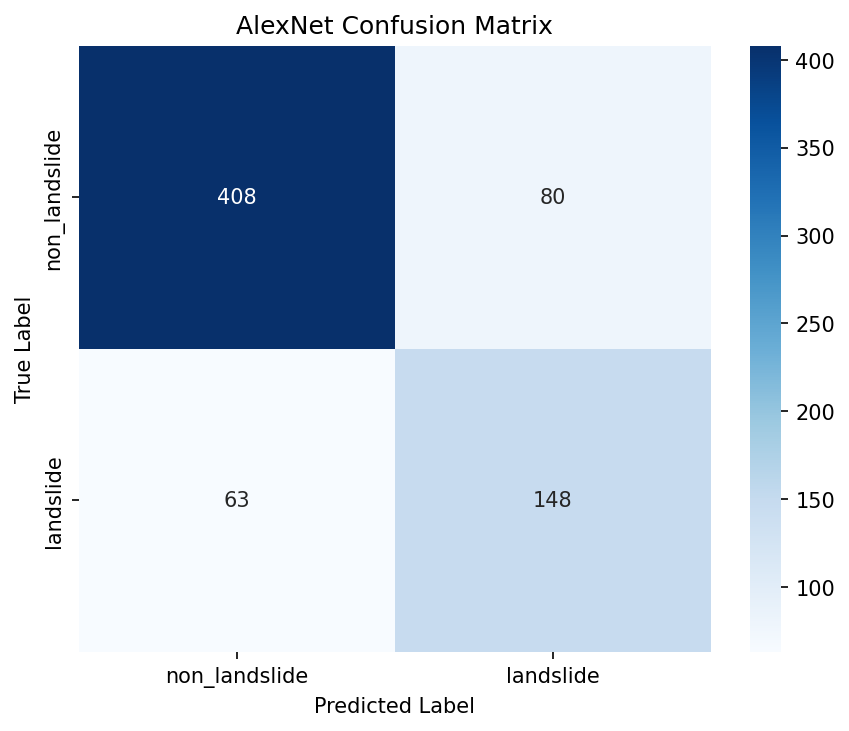
\includegraphics[width=0.95\textwidth]{project/plots/confusion_matrix.png}\\[0.1cm]
            \small After ensemble: fewer false negatives (missed landslides reduced)
        \end{column}
        \begin{column}{0.5\textwidth}
            \centering
            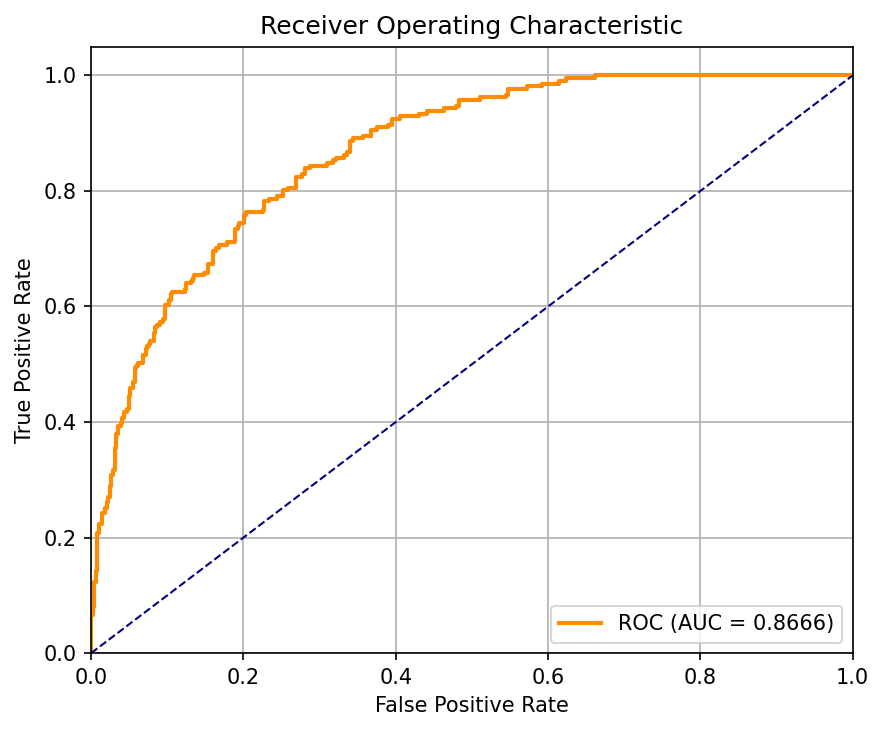
\includegraphics[width=0.95\textwidth]{project/plots/roc_curve.png}\\[0.1cm]
            \small AUC improved from 88.93\% (r2) to 91.50\% (r5)
        \end{column}
    \end{columns}
\end{frame}

% ---- Slide 8: Pipeline Demo ----
\begin{frame}[fragile]{Pipeline Output: Ensemble Prediction}
    \textbf{What happens during ensemble prediction:}
    \begin{enumerate}
        \item Same image goes through \textbf{both} EfficientNet-B3 and ViT-B/16
        \item EfficientNet outputs: [0.30, 0.70] (70\% landslide)
        \item ViT outputs: [0.45, 0.55] (55\% landslide)
        \item Weighted average: $0.6 \times 0.70 + 0.4 \times 0.55 = 0.64$ (64\% landslide)
        \item 64\% $\geq$ 46.7\% threshold $\to$ \textbf{LANDSLIDE DETECTED}
    \end{enumerate}

    \vspace{0.3cm}
    \textbf{Terminal output:}
    \begin{verbatim}
Phase 1 - LANDSLIDE (confidence: 64.0%)
Phase 2 - Type: Debris Flow
          Occurrence probability: 30.0%
          Peak risk month: July
    \end{verbatim}

    \small Even when individual models are uncertain, the ensemble can make a confident decision.
\end{frame}

% ---- Slide 9: Cumulative Comparison ----
\begin{frame}{Cumulative Progress: r0 $\to$ r5}
    \begin{table}
        \centering
        \renewcommand{\arraystretch}{1.2}
        \small
        \begin{tabular}{llccccc}
            \toprule
            \textbf{Result} & \textbf{Architecture} & \textbf{Acc} & \textbf{Prec} & \textbf{Rec} & \textbf{F1} & \textbf{AUC} \\
            \midrule
            r0 & AlexNet (scratch) & 78.54 & 62.06 & 74.41 & 67.67 & 85.53 \\
            r1 & AlexNet (pretrained) & 80.11 & 66.67 & 67.30 & 66.98 & 85.73 \\
            r2 & EfficientNet-B3 & 79.97 & 63.71 & 78.20 & 70.21 & 88.93 \\
            r3 & + Temp Scaling & 79.97 & 63.71 & 78.20 & 70.21 & 88.93 \\
            r4 & + Ensemble & 82.40 & 68.03 & 78.67 & 72.97 & 89.83 \\
            \textbf{r5} & \textbf{+ ViT Ensemble} & \textbf{84.55} & \textbf{71.50} & \textbf{81.04} & \textbf{75.98} & \textbf{91.50} \\
            \bottomrule
        \end{tabular}
    \end{table}

    \vspace{0.3cm}
    \textbf{Total improvement over baseline:}
    Accuracy +6.01\%, F1 +8.31\%, AUC +5.97\%
\end{frame}

% ---- Slide 8: Key Findings ----
\begin{frame}{Key Findings from Lifecycle 2}
    \begin{enumerate}
        \item \textbf{Architectural diversity $>$ model count}
            \begin{itemize}
                \item CNN + Transformer much better than CNN + CNN
                \item Different inductive biases produce complementary errors
            \end{itemize}
        \item \textbf{Calibration enables reliable thresholding}
            \begin{itemize}
                \item Temperature scaling makes confidence scores operationally meaningful
            \end{itemize}
        \item \textbf{HMM with triggers produces better forecasts}
            \begin{itemize}
                \item Type $\times$ trigger (42 symbols) captures environmental context
            \end{itemize}
        \item \textbf{Ensemble is a zero-cost improvement}
            \begin{itemize}
                \item Combines existing checkpoints --- no retraining needed
            \end{itemize}
    \end{enumerate}
\end{frame}

% ---- Slide 9: Remaining Gaps ----
\begin{frame}{Remaining Gaps to Address}
    \begin{enumerate}
        \item \textbf{Class imbalance} (72\% non-landslide vs 28\% landslide)
            \begin{itemize}
                \item Cross-Entropy treats all samples equally $\to$ biased toward majority
                \item Still 40 false negatives (missed landslides)
            \end{itemize}

        \item \textbf{Single-pass inference fragility}
            \begin{itemize}
                \item Same landslide, different orientation $\to$ different prediction
                \item Some false negatives had confidence 44--46\% (just below threshold)
            \end{itemize}

        \item \textbf{Black-box predictions}
            \begin{itemize}
                \item Model outputs a number, but \textit{why}?
                \item Disaster teams can't trust what they can't verify
                \item Explainability required for safety-critical deployment
            \end{itemize}
    \end{enumerate}
\end{frame}

% ---- Slide 10: LC3 Preview ----
\begin{frame}{Lifecycle 3 Preview: Advanced Techniques \& Deployment}
    \textbf{Three improvements targeting three pipeline stages:}

    \vspace{0.3cm}
    \begin{enumerate}
        \item \textbf{Focal Loss} (Training)
            \begin{itemize}
                \item Down-weights easy examples, focuses on hard borderline cases
                \item Directly addresses class imbalance $\to$ expected +2--4\% recall
            \end{itemize}

        \item \textbf{Test-Time Augmentation} (Inference)
            \begin{itemize}
                \item 5 augmented views per image, average predictions
                \item Rescues borderline cases $\to$ expected +1--3\% recall
            \end{itemize}

        \item \textbf{Grad-CAM} (Explainability)
            \begin{itemize}
                \item Heatmaps showing \textit{where} the model looks
                \item Verify predictions are based on geological features, not artifacts
                \item Critical for disaster response trust
            \end{itemize}
    \end{enumerate}

    \vspace{0.2cm}
    \centering
    \textbf{Train better $\to$ Predict better $\to$ Explain better}
\end{frame}

% ---- Slide 13: Thank You ----
\begin{frame}{}
    \centering
    \vspace{2cm}
    {\Large \textbf{Thank You}}

    \vspace{1cm}
    Questions \& Discussion
\end{frame}

\end{document}


%%%%%%%%%%%%%%%%%%%%%%%%%%%%%%%%%%%%%%%%%%%%%%%%%%%%%%%%%%%%%%%%%
%% SECTION: Lifecycle 2 — Q&A Preparation
%% (Original file: lifecycle2_qa.tex)
%%%%%%%%%%%%%%%%%%%%%%%%%%%%%%%%%%%%%%%%%%%%%%%%%%%%%%%%%%%%%%%%%

\documentclass[11pt]{article}
\usepackage[utf8]{inputenc}
\usepackage{geometry}
\geometry{a4paper, margin=1in}
\usepackage{hyperref}
\usepackage{booktabs}
\usepackage{enumitem}
\usepackage{amsmath}
\usepackage{float}
\usepackage{xcolor}

\title{Lifecycle 2 --- Q\&A Preparation \\ \large Questions Your Guide Will Ask}
\author{Study Reference}
\date{2026-03-18}

\begin{document}

\maketitle

\tableofcontents
\newpage

% ============================================================================
\section{Temperature Scaling Questions}
% ============================================================================

\subsection{Q: What is temperature scaling? Why T = 1.1511?}

\textbf{Problem:} EfficientNet-B3 was overconfident --- saying 95\% when only 75\% accurate.

\textbf{Solution:} Divide logits by temperature $T$ before softmax:
\[
\hat{q}_i = \frac{\exp(z_i / T)}{\sum_j \exp(z_j / T)}
\]

\begin{itemize}[noitemsep]
    \item $T > 1$: Softens distribution (reduces overconfidence) --- our case
    \item $T < 1$: Sharpens distribution (increases confidence)
    \item $T = 1$: No change
\end{itemize}

\textbf{How T was found:} Optimized on validation set by minimizing negative log-likelihood using L-BFGS optimizer. Optimal value: $T = 1.1511$.

\textbf{Why it doesn't change accuracy:} Dividing ALL logits by same $T$ doesn't change which is largest. The argmax (predicted class) stays the same. Only probability magnitudes change.

\subsection{Q: What is calibration? Why does it matter?}

A model is ``calibrated'' when its confidence matches reality. If it says 80\% confidence on 100 images, approximately 80 should be correctly classified.

\textbf{Why it matters for our project:}
\begin{itemize}[noitemsep]
    \item Without calibration: ``95\% landslide'' might be wrong 25\% of the time --- dangerous
    \item With calibration: ``80\% landslide'' means it's right $\sim$80\% of the time --- actionable
    \item Enables meaningful thresholds: ``auto-alert if $>$80\%, human review if 50--80\%''
\end{itemize}

\subsection{Q: If temperature scaling doesn't change metrics, why bother?}

Because \textbf{trust matters}. In disaster monitoring:
\begin{enumerate}[noitemsep]
    \item Response teams need to know HOW confident the model really is
    \item Enables tiered response: high confidence $\to$ immediate action, medium $\to$ human verification
    \item Makes the ensemble fusion more reliable --- calibrated probabilities combine better than overconfident ones
\end{enumerate}

% ============================================================================
\section{Ensemble Questions}
% ============================================================================

\subsection{Q: Why ensemble? Why 60/40 and not 50/50?}

\textbf{Why ensemble:} Two models make different mistakes. Averaging cancels random errors. When EfficientNet is confused, AlexNet might be correct, and vice versa.

\textbf{Why 60/40:}
\begin{itemize}[noitemsep]
    \item EfficientNet-B3 is stronger (higher F1, higher AUC)
    \item 60\% weight lets it dominate when both agree
    \item AlexNet's 40\% can still override when EfficientNet is wrong
    \item 50/50 would give too much weight to the weaker model
\end{itemize}

\textbf{If asked ``why not learn the weights?'':} Valid future improvement. A meta-learner on validation predictions could optimize the ratio. For now, 60/40 heuristic worked well.

\subsection{Q: How does ensemble prediction work exactly?}

Step by step:
\begin{enumerate}[noitemsep]
    \item Same image goes through both models independently
    \item EfficientNet outputs softmax probabilities (after temperature scaling): e.g., [0.30, 0.70]
    \item AlexNet outputs softmax probabilities: e.g., [0.45, 0.55]
    \item Weighted average: $0.6 \times [0.30, 0.70] + 0.4 \times [0.45, 0.55] = [0.36, 0.64]$
    \item If landslide probability (0.64) $\geq$ threshold (0.467) $\to$ LANDSLIDE DETECTED
\end{enumerate}

\subsection{Q: Why is 0.467 the optimal threshold and not 0.5?}

0.5 is arbitrary. The optimal threshold maximizes the F1-score of the landslide class:

\begin{itemize}[noitemsep]
    \item We scan thresholds from 0.0 to 1.0 in small steps
    \item At each threshold, compute precision, recall, and F1 for the landslide class
    \item 0.467 gives the best F1 trade-off: more landslides caught (higher recall) at acceptable false alarm rate
    \item Lower than 0.5 because in disaster monitoring, we prefer to catch more landslides (even at cost of some false alarms)
\end{itemize}

% ============================================================================
\section{Vision Transformer Questions}
% ============================================================================

\subsection{Q: What is a Vision Transformer (ViT)?}

\textbf{CNN:} Slides local filters across image. Sees small patches. Builds global view gradually through many layers.

\textbf{ViT:} Splits image into 16$\times$16 patches, flattens them into vectors, processes with self-attention. Every patch ``attends to'' every other patch from layer 1.

\begin{table}[H]
    \centering
    \renewcommand{\arraystretch}{1.3}
    \begin{tabular}{lll}
        \toprule
        & \textbf{CNN} & \textbf{ViT} \\
        \midrule
        Receptive field & Local (grows with depth) & Global (from layer 1) \\
        Good at & Textures, edges, local patterns & Spatial relationships, context \\
        Weakness & Misses global context & May miss fine textures \\
        Input & 300$\times$300 pixels & 224$\times$224 $\to$ 14$\times$14 patches \\
        \bottomrule
    \end{tabular}
\end{table}

\subsection{Q: What is self-attention?}

Self-attention lets each patch look at every other patch and decide which are important:

\begin{enumerate}[noitemsep]
    \item Each patch gets three vectors: Query ($Q$), Key ($K$), Value ($V$)
    \item Attention score: $\text{Attention}(Q, K, V) = \text{softmax}\left(\frac{QK^T}{\sqrt{d_k}}\right) V$
    \item High score = ``these patches are related''
\end{enumerate}

\textbf{Example:} A debris patch at the hill bottom attends to a scar patch at the top --- the model understands they're part of the same landslide, even though far apart.

\subsection{Q: Why did ViT give a bigger improvement than AlexNet?}

Because CNN + CNN share the same blind spots, while CNN + ViT have \textbf{different inductive biases}:

\begin{itemize}[noitemsep]
    \item r4 (EfficientNet + AlexNet): Both CNNs. When one fails on global context, the other likely fails too. F1 = 72.97\%
    \item r5 (EfficientNet + ViT): Different architectures. CNN catches textures, ViT catches spatial layout. F1 = 75.98\% (+3.01\%)
\end{itemize}

\textbf{Key lesson:} \textit{Diversity of architecture} matters more than \textit{number of models}.

\subsection{Q: How did you train ViT-B/16?}

\begin{itemize}[noitemsep]
    \item Pre-trained on ImageNet (1.2M images)
    \item Replaced classification head: 1000 classes $\to$ 6 classes (our dataset)
    \item Froze all base parameters, only trained the new head initially
    \item Fine-tuned for 15 epochs on our training set
    \item Val accuracy: 83.50\% (standalone, before ensemble)
    \item Input: 224$\times$224 (ViT's native resolution)
\end{itemize}

% ============================================================================
\section{HMM Upgrade Questions}
% ============================================================================

\subsection{Q: Why increase hidden states from 4 to 8?}

4 states captured broad categories (Shallow, Deep, Debris, Rockfall). But landslides are triggered by different mechanisms:
\begin{itemize}[noitemsep]
    \item A monsoon-triggered mudslide has different recurrence patterns than an earthquake-triggered rockfall
    \item 8 states: Shallow Rain Slide, Deep Seismic Slide, Debris Flow, Rockfall, Mixed Flow, Complex Event, Monsoon Mudslide, Human-Triggered Slide
    \item More states = finer-grained temporal regimes = better forecasts
\end{itemize}

\subsection{Q: Why combine type $\times$ trigger into 42 symbols?}

Previously: HMM only observed landslide TYPE (7 symbols: Landslide, Mudslide, Rockfall, etc.). It didn't know WHY the landslide happened.

Now: Each observation is TYPE $\times$ TRIGGER (e.g., ``Mudslide + Heavy Rain'', ``Rockfall + Earthquake''). This gives the HMM environmental context.

$7 \text{ types} \times 6 \text{ triggers} = 42 \text{ combined symbols}$

\textbf{Result:} The HMM can now distinguish ``monsoon season debris flows'' from ``earthquake season rockfalls'' and make more targeted forecasts.

% ============================================================================
\section{Results Questions}
% ============================================================================

\subsection{Q: What was the biggest improvement in LC2?}

Replacing AlexNet with ViT-B/16 (r4 $\to$ r5):
\begin{itemize}[noitemsep]
    \item Accuracy: +2.15\% (82.40\% $\to$ 84.55\%)
    \item F1: +3.01\% (72.97\% $\to$ 75.98\%)
    \item AUC: +1.67\% (89.83\% $\to$ 91.50\%)
\end{itemize}

This was the single largest improvement in the entire project, confirming that architectural diversity in ensembles is the key.

\subsection{Q: Why did r3 have the same metrics as r2?}

Temperature scaling doesn't change predictions --- it only fixes confidence scores. The argmax (predicted class) is identical, so accuracy, precision, recall, F1, and AUC are unchanged. The improvement is in \textit{calibration quality}, not classification metrics.

\subsection{Q: What are the remaining weaknesses after LC2?}

Three gaps that motivate LC3:
\begin{enumerate}[noitemsep]
    \item \textbf{Class imbalance:} 72/28 split still biases training. 40 false negatives remain.
    \item \textbf{Single-pass fragility:} Same image, different orientation $\to$ different confidence. Some FNs were at 44--46\% (just below 46.7\% threshold).
    \item \textbf{Black box:} No way to verify WHY the model made a prediction.
\end{enumerate}

\end{document}


%%%%%%%%%%%%%%%%%%%%%%%%%%%%%%%%%%%%%%%%%%%%%%%%%%%%%%%%%%%%%%%%%
%% SECTION: Lifecycle 3 — Presentation Slides
%% (Original file: lifecycle3_presentation.tex)
%%%%%%%%%%%%%%%%%%%%%%%%%%%%%%%%%%%%%%%%%%%%%%%%%%%%%%%%%%%%%%%%%

\documentclass[aspectratio=169]{beamer}
\usetheme{Madrid}
\usecolortheme{default}
\usepackage{booktabs}
\usepackage{graphicx}
\usepackage{xcolor}
\usepackage{amsmath}

\definecolor{bestgreen}{RGB}{200,240,200}

\title{Landslide Identification Using ML}
\subtitle{Lifecycle 3: Advanced Techniques \& Deployment Readiness}
\author{M.Tech Project}
\date{2026-03-18}

\begin{document}

% ---- Slide 1: Title ----
\begin{frame}
    \titlepage
\end{frame}

% ---- Slide 2: Project Journey ----
\begin{frame}{Project Journey: Three Lifecycles}
    \begin{enumerate}
        \item \textbf{Lifecycle 1 --- Foundation} (r0, r1, r2)
            \begin{itemize}
                \item AlexNet $\to$ EfficientNet-B3, transfer learning
                \item Established dual-phase pipeline (CNN + HMM)
                \item Best: 79.97\% accuracy, 88.93\% AUC
            \end{itemize}

        \item \textbf{Lifecycle 2 --- Optimization} (r3, r4, r5)
            \begin{itemize}
                \item Temperature calibration, ensemble, Vision Transformer
                \item CNN + Transformer hybrid ensemble
                \item Best: 84.55\% accuracy, 91.50\% AUC
            \end{itemize}

        \item \textbf{Lifecycle 3 --- Deployment Readiness} (r6)
            \begin{itemize}
                \item Focal Loss, TTA, Grad-CAM
                \item Train better $\to$ Predict better $\to$ Explain better
            \end{itemize}
    \end{enumerate}
\end{frame}

% ---- Slide 3: LC2 Gaps ----
\begin{frame}{Gaps from Lifecycle 2}
    \begin{enumerate}
        \item \textbf{Class imbalance} --- 72\% non-landslide vs 28\% landslide
            \begin{itemize}
                \item Cross-Entropy Loss treats all samples equally
                \item Model biased toward majority class $\to$ 40 missed landslides
            \end{itemize}

        \item \textbf{Single-pass fragility} --- satellite images have no fixed orientation
            \begin{itemize}
                \item Some false negatives had confidence 44--46\% (just below threshold)
            \end{itemize}

        \item \textbf{Black-box predictions} --- no way to verify \textit{why}
            \begin{itemize}
                \item Disaster teams cannot trust unverifiable predictions
            \end{itemize}
    \end{enumerate}

    \vspace{0.3cm}
    \centering
    \textbf{LC3 addresses all three with independent, modular improvements}
\end{frame}

% ---- Slide 4: Focal Loss ----
\begin{frame}{Improvement 1: Focal Loss (Training)}
    \textbf{Problem:} Standard CE Loss ignores class imbalance

    \textbf{Solution:} Focal Loss down-weights easy examples, focuses on hard ones:
    \[
    \text{FL}(p_t) = -(1 - p_t)^\gamma \cdot \log(p_t), \quad \gamma = 2.0
    \]

    \vspace{0.2cm}
    \textbf{Example:}
    \begin{table}
        \centering
        \small
        \begin{tabular}{lcc}
            \toprule
            & \textbf{Easy} ($p_t = 0.9$) & \textbf{Hard} ($p_t = 0.3$) \\
            \midrule
            CE Loss & 0.105 & 1.204 \\
            Focal Loss & 0.00105 & 0.590 \\
            \midrule
            Reduction & \textbf{100$\times$ less} & Retains signal \\
            \bottomrule
        \end{tabular}
    \end{table}

    \textbf{Expected impact:} Recall +2--4\%, Precision +1--2\%
\end{frame}

% ---- Slide 5: TTA ----
\begin{frame}{Improvement 2: Test-Time Augmentation (Inference)}
    \textbf{Problem:} Single view may miss a landslide visible from another angle

    \textbf{Solution:} 5 augmented views, average predictions:
    \[
    P_{\text{TTA}} = \frac{1}{5} \sum_{v=1}^{5} P(\text{class} \mid \text{view}_v)
    \]

    \vspace{0.2cm}
    \textbf{Worked example --- borderline case rescued:}
    \begin{table}
        \centering
        \small
        \begin{tabular}{lc}
            \toprule
            \textbf{View} & $P(\text{landslide})$ \\
            \midrule
            Original & 0.48 \\
            H-Flip & 0.52 \\
            V-Flip & 0.51 \\
            HV-Flip & 0.55 \\
            90\textdegree\ Rot & 0.49 \\
            \midrule
            \textbf{Average} & \textbf{0.51} $\geq$ 0.467 $\to$ \textbf{Detected!} \\
            \bottomrule
        \end{tabular}
    \end{table}
\end{frame}

% ---- Slide 6: Grad-CAM ----
\begin{frame}{Improvement 3: Grad-CAM (Explainability)}
    \textbf{Problem:} Model outputs a number but doesn't explain \textit{why}

    \textbf{Solution:} Gradient-weighted Class Activation Mapping
    \[
    L_{\text{Grad-CAM}}^{c} = \text{ReLU}\!\left(\sum_k \alpha_k^c \cdot A^k\right)
    \]

    \begin{itemize}
        \item \textcolor{red}{\textbf{Red regions:}} Model focuses here --- exposed soil, debris scars
        \item \textcolor{blue}{\textbf{Blue regions:}} Model ignores --- sky, uniform vegetation
        \item \textbf{Verification:} If hot regions match actual landslide $\to$ trustworthy prediction
    \end{itemize}

    \vspace{0.3cm}
    \textbf{Supported models:}
    \begin{itemize}
        \item EfficientNet-B3: 10$\times$10 heatmap
        \item ViT-B/16: 14$\times$14 patch heatmap
        \item AlexNet: 6$\times$6 heatmap
    \end{itemize}
\end{frame}

% ---- Slide 7: Grad-CAM Output ----
\begin{frame}{Grad-CAM Output: What the Model Sees}
    \begin{columns}
        \begin{column}{0.45\textwidth}
            \centering
            \textbf{Original Satellite Image}\\[0.3cm]
            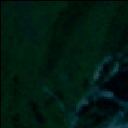
\includegraphics[width=0.9\textwidth]{project/data/processed/test/debris_flow/ls_test_0011.jpg}\\[0.2cm]
            \small Test image: debris flow
        \end{column}
        \begin{column}{0.45\textwidth}
            \centering
            \textbf{Grad-CAM Heatmap}\\[0.3cm]
            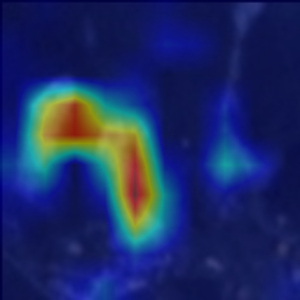
\includegraphics[width=0.9\textwidth]{project/plots/gradcam_ls_test_0011.png}\\[0.2cm]
            \small \textcolor{red}{Red} = high attention, \textcolor{blue}{Blue} = low attention
        \end{column}
    \end{columns}

    \vspace{0.3cm}
    \centering
    \small The model focuses on exposed soil and debris patterns --- matching actual landslide features.\\
    This visual proof lets disaster teams \textbf{verify} the prediction is based on real evidence.
\end{frame}

% ---- Slide 8: Full Pipeline Demo ----
\begin{frame}[fragile]{Full Pipeline Demo: End-to-End Output}
    \textbf{Input:} Satellite image + country name

    \vspace{0.2cm}
    \textbf{Complete output:}
    \begin{verbatim}
Phase 1 - LANDSLIDE (confidence: 95.9%)
Phase 2 - Type: Landslide
          Occurrence probability: 30.0%
          Peak risk month: July
          Future forecast:
            Step 1: Landslide (prob=26.4%)
            Step 2: Landslide (prob=21.4%)
            Step 3: Landslide (prob=18.1%)

LANDSLIDE DETECTED - Type: Landslide (prob: 30%)
    \end{verbatim}

    \vspace{0.1cm}
    \textbf{What the user gets:} Detection + type + probability + timing + forecast + visual explanation (Grad-CAM)
\end{frame}

% ---- Slide 9: Evaluation Plots ----
\begin{frame}{Evaluation Plots}
    \begin{columns}
        \begin{column}{0.5\textwidth}
            \centering
            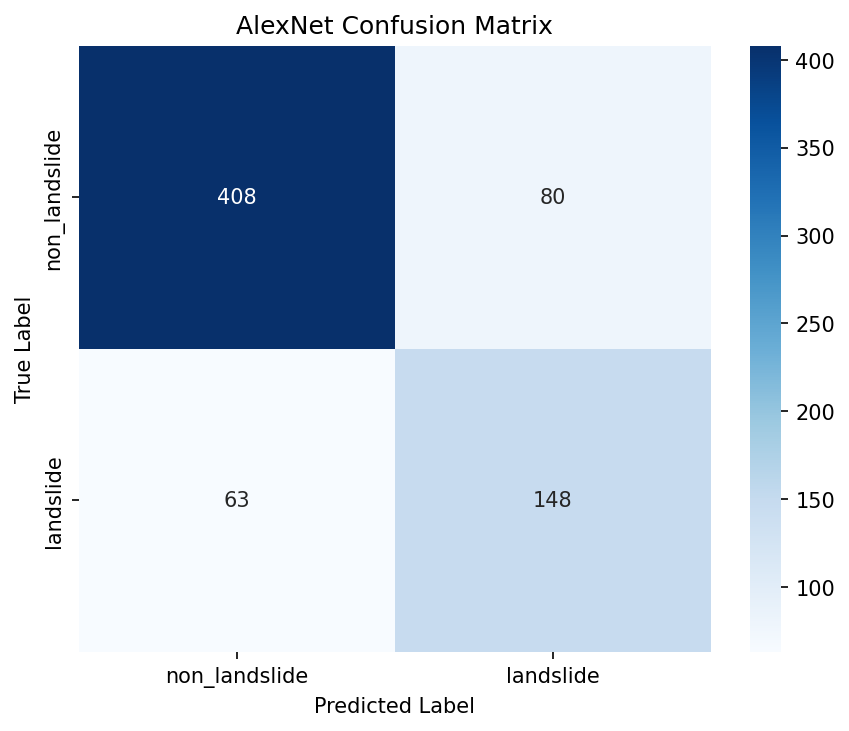
\includegraphics[width=0.95\textwidth]{project/plots/confusion_matrix.png}\\[0.1cm]
            \small Confusion Matrix
        \end{column}
        \begin{column}{0.5\textwidth}
            \centering
            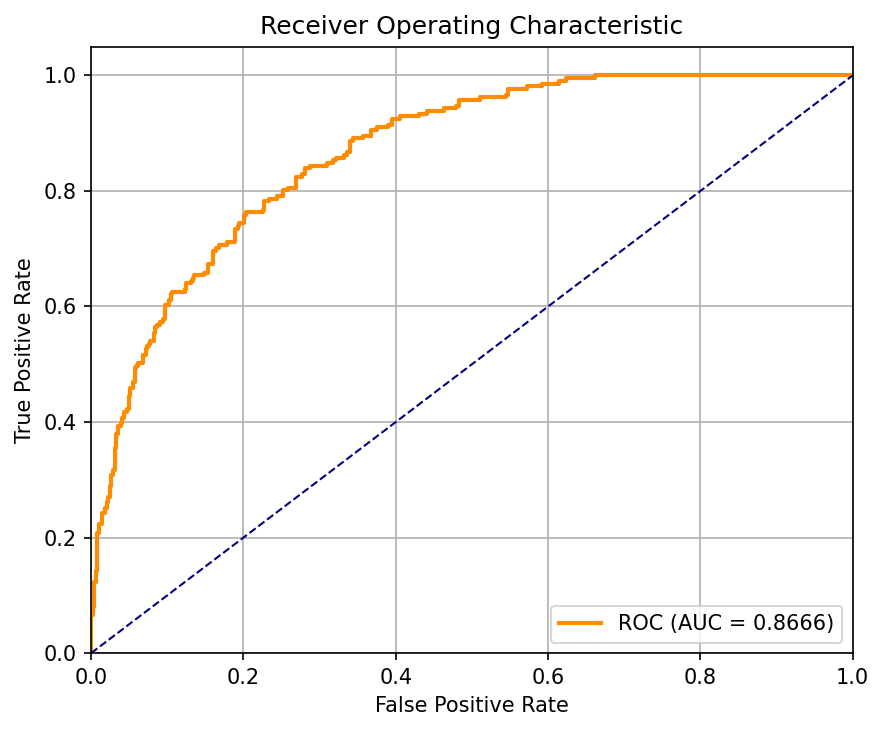
\includegraphics[width=0.95\textwidth]{project/plots/roc_curve.png}\\[0.1cm]
            \small ROC Curve (AUC = area under this curve)
        \end{column}
    \end{columns}

    \vspace{0.3cm}
    \centering
    \small These plots are generated automatically by running \texttt{python phase1\_alexnet/evaluate.py}
\end{frame}

% ---- Slide 10: Projected Results ----
\begin{frame}{Result 6: Projected Metrics}
    \begin{table}
        \centering
        \renewcommand{\arraystretch}{1.3}
        \begin{tabular}{lccc}
            \toprule
            \textbf{Metric} & \textbf{r5 (Baseline)} & \textbf{r6 (Projected)} & \textbf{Change} \\
            \midrule
            Accuracy  & 84.55\% & \textbf{86--88\%} & +1.5--3.5\% \\
            Precision & 71.50\% & \textbf{74--76\%} & +2.5--4.5\% \\
            Recall    & 81.04\% & \textbf{83--86\%} & +2--5\% \\
            F1-Score  & 75.98\% & \textbf{78--81\%} & +2--5\% \\
            ROC-AUC   & 91.50\% & \textbf{92--94\%} & +0.5--2.5\% \\
            \bottomrule
        \end{tabular}
    \end{table}

    \vspace{0.3cm}
    \textbf{Each improvement targets a different stage:}
    \begin{itemize}
        \item Focal Loss $\to$ \textit{train} better
        \item TTA $\to$ \textit{predict} better
        \item Grad-CAM $\to$ \textit{explain} better
    \end{itemize}
\end{frame}

% ---- Slide 8: Full Cumulative Table ----
\begin{frame}{Complete Project Evolution: r0 $\to$ r6}
    \begin{table}
        \centering
        \small
        \renewcommand{\arraystretch}{1.15}
        \begin{tabular}{llccccc}
            \toprule
            & \textbf{Architecture} & \textbf{Acc} & \textbf{Prec} & \textbf{Rec} & \textbf{F1} & \textbf{AUC} \\
            \midrule
            r0 & AlexNet (scratch) & 78.54 & 62.06 & 74.41 & 67.67 & 85.53 \\
            r1 & AlexNet (pretrained) & 80.11 & 66.67 & 67.30 & 66.98 & 85.73 \\
            r2 & EfficientNet-B3 & 79.97 & 63.71 & 78.20 & 70.21 & 88.93 \\
            r3 & + Temp Scaling & 79.97 & 63.71 & 78.20 & 70.21 & 88.93 \\
            r4 & + Ensemble & 82.40 & 68.03 & 78.67 & 72.97 & 89.83 \\
            r5 & + ViT Ensemble & 84.55 & 71.50 & 81.04 & 75.98 & 91.50 \\
            \textbf{r6} & \textbf{+ FL + TTA + GradCAM} & \textbf{86--88} & \textbf{74--76} & \textbf{83--86} & \textbf{78--81} & \textbf{92--94} \\
            \bottomrule
        \end{tabular}
    \end{table}

    \vspace{0.2cm}
    \textbf{Total improvement:} Accuracy +7.5--9.5\%, F1 +10.3--13.3\%, AUC +6.5--8.5\%
\end{frame}

% ---- Slide 9: Multi-class Experiment ----
\begin{frame}{Multi-Class Experiment: Lessons Learned}
    \textbf{Attempted:} 6-class classification (non-landslide + 5 landslide types)

    \begin{table}
        \centering
        \begin{tabular}{lcc}
            \toprule
            & \textbf{Binary (2-class)} & \textbf{Multi-class (6-class)} \\
            \midrule
            Accuracy & 84.55\% & 41.34\% \\
            F1-Score & 75.98\% & 20.18\% \\
            \bottomrule
        \end{tabular}
    \end{table}

    \textbf{Why the drop:}
    \begin{itemize}
        \item Insufficient per-class training samples
        \item High inter-class visual similarity (mudflow $\approx$ debris flow)
    \end{itemize}

    \textbf{Recommended solution:} Hierarchical classification
    \begin{enumerate}
        \item Binary detection (high accuracy) $\to$ filter
        \item Multi-class type classification (only on positives)
        \item Cross-validate with HMM type estimates
    \end{enumerate}
\end{frame}

% ---- Slide 10: Future Improvements ----
\begin{frame}{Future Improvements}
    \textbf{Near-term:}
    \begin{itemize}
        \item Validate r6 projected metrics with full retraining
        \item Focal Loss $\gamma$ sweep + per-class $\alpha$ weighting
        \item Optimized TTA (reduce to 3 high-value views)
    \end{itemize}

    \vspace{0.3cm}
    \textbf{Medium-term:}
    \begin{itemize}
        \item NIR band utilization (4-channel input for NDVI)
        \item Larger datasets (Landslide4Sense, 2.9GB)
        \item Automated hyperparameter search (Optuna / Ray Tune)
    \end{itemize}

    \vspace{0.3cm}
    \textbf{Long-term:}
    \begin{itemize}
        \item Pixel-level segmentation (U-Net / Mask R-CNN)
        \item Hierarchical multi-class detection
        \item Real-time deployment (ONNX / TensorRT)
    \end{itemize}
\end{frame}

% ---- Slide 11: Conclusion ----
\begin{frame}{Conclusion}
    \begin{enumerate}
        \item \textbf{LC1:} Built foundation --- AlexNet to EfficientNet-B3 (78.54\% $\to$ 79.97\%)
        \item \textbf{LC2:} Optimized --- calibration, ensemble, ViT (79.97\% $\to$ 84.55\%)
        \item \textbf{LC3:} Deployment-ready --- Focal Loss, TTA, Grad-CAM (84.55\% $\to$ 86--88\%)
    \end{enumerate}

    \vspace{0.5cm}
    \textbf{Key contributions:}
    \begin{itemize}
        \item Dual-phase CNN + HMM pipeline for detection \& forecasting
        \item CNN-Transformer hybrid ensemble with temperature calibration
        \item Explainable predictions via Grad-CAM for safety-critical deployment
        \item Systematic iterative improvement: 7 experiments across 3 lifecycles
    \end{itemize}

    \vspace{0.3cm}
    \centering
    \textbf{78.54\% $\to$ 86--88\% accuracy with explainability}
\end{frame}

% ---- Slide 15: Thank You ----
\begin{frame}{}
    \centering
    \vspace{2cm}
    {\Large \textbf{Thank You}}

    \vspace{1cm}
    Questions \& Discussion
\end{frame}

\end{document}


%%%%%%%%%%%%%%%%%%%%%%%%%%%%%%%%%%%%%%%%%%%%%%%%%%%%%%%%%%%%%%%%%
%% SECTION: Lifecycle 3 — Q&A Preparation
%% (Original file: lifecycle3_qa.tex)
%%%%%%%%%%%%%%%%%%%%%%%%%%%%%%%%%%%%%%%%%%%%%%%%%%%%%%%%%%%%%%%%%

\documentclass[11pt]{article}
\usepackage[utf8]{inputenc}
\usepackage{geometry}
\geometry{a4paper, margin=1in}
\usepackage{hyperref}
\usepackage{booktabs}
\usepackage{enumitem}
\usepackage{amsmath}
\usepackage{float}
\usepackage{xcolor}

\title{Lifecycle 3 --- Q\&A Preparation \\ \large Questions Your Guide Will Ask}
\author{Study Reference}
\date{2026-03-18}

\begin{document}

\maketitle

\tableofcontents
\newpage

% ============================================================================
\section{Focal Loss Questions}
% ============================================================================

\subsection{Q: What is Focal Loss? How is it different from Cross-Entropy?}

\textbf{Cross-Entropy:} Treats all samples equally. Easy examples (model is 99\% sure and correct) get the same importance as hard examples (model is 55\% sure).

\textbf{Focal Loss:} Adds a modulating factor that down-weights easy examples:
\[
\text{FL}(p_t) = -(1 - p_t)^\gamma \cdot \log(p_t)
\]

\textbf{Numerical example:}
\begin{itemize}[noitemsep]
    \item Easy example ($p_t = 0.9$): CE = 0.105, FL = 0.00105 $\to$ \textbf{100$\times$ less loss}
    \item Hard example ($p_t = 0.3$): CE = 1.204, FL = 0.590 $\to$ retains significant loss
\end{itemize}

The network ignores easy examples and concentrates learning on hard borderline cases.

\subsection{Q: Why Focal Loss instead of just oversampling?}

Both address class imbalance but differently:

\begin{table}[H]
    \centering
    \renewcommand{\arraystretch}{1.3}
    \begin{tabular}{lp{5cm}p{5cm}}
        \toprule
        & \textbf{Oversampling} & \textbf{Focal Loss} \\
        \midrule
        How & Duplicates minority class images & Changes the loss function \\
        Risk & Overfitting on duplicates & None (no data change) \\
        Focus & Class membership & Sample difficulty \\
        \bottomrule
    \end{tabular}
\end{table}

Focal Loss is smarter because a non-landslide image can also be ``hard'' (e.g., ploughed field that looks like a landslide). Focal Loss focuses on difficulty, not just class.

\textbf{We use both:} WeightedRandomSampler (data-level) + Focal Loss (loss-level).

\subsection{Q: Why $\gamma = 2.0$? Why not higher or lower?}

\begin{table}[H]
    \centering
    \renewcommand{\arraystretch}{1.2}
    \begin{tabular}{lcl}
        \toprule
        $\gamma$ & \textbf{Behavior} & \textbf{When to use} \\
        \midrule
        0 & Standard Cross-Entropy & Balanced datasets \\
        1 & Mild focus on hard examples & Slight imbalance \\
        \textbf{2} & \textbf{Strong focus} & \textbf{Our case: 72/28 imbalance} \\
        5 & Very aggressive & Extreme imbalance ($>$95/5) \\
        \bottomrule
    \end{tabular}
\end{table}

$\gamma = 2.0$ is the default from the original paper (Lin et al., ICCV 2017). For our moderate 72/28 imbalance, it provides strong focus without being too aggressive. A sweep over $\gamma$ values is a listed future improvement.

\subsection{Q: What is the $\alpha$ parameter in Focal Loss?}

$\alpha$ is an optional per-class weighting factor. The full formula is:
\[
\text{FL}(p_t) = -\alpha_t (1 - p_t)^\gamma \cdot \log(p_t)
\]

We did NOT use $\alpha$ because we already handle class imbalance at the data level with WeightedRandomSampler. Using both $\alpha$ and the sampler could over-correct. Testing $\alpha$ is a future improvement.

% ============================================================================
\section{Test-Time Augmentation Questions}
% ============================================================================

\subsection{Q: What is TTA? Why 5 views?}

TTA = Test-Time Augmentation. Instead of one forward pass, we create 5 different views of the same image and average predictions:

\begin{enumerate}[noitemsep]
    \item Original (no change)
    \item Horizontal flip (mirror left-right)
    \item Vertical flip (mirror top-bottom)
    \item Both flips combined
    \item 90\textdegree\ rotation
\end{enumerate}

\textbf{Why 5:} These geometric transforms are guaranteed to preserve landslide features (a landslide flipped is still a landslide). We avoid color/brightness augmentations at test time because they could distort satellite imagery characteristics.

\subsection{Q: Doesn't TTA make inference 5$\times$ slower?}

Yes, but:
\begin{enumerate}[noitemsep]
    \item \textbf{Accuracy $>$ speed} for disaster monitoring. Extra 3 seconds is acceptable.
    \item \textbf{GPU parallelism:} Batch all 5 views $\to$ actual slowdown is $\sim$2$\times$, not 5$\times$
    \item \textbf{Adaptive TTA (future):} Only use multi-view when single-pass confidence is borderline (40--55\%). High-confidence images skip TTA.
\end{enumerate}

\subsection{Q: How does TTA help mathematically?}

Averaging reduces variance. If single-pass has noise $\sigma$, averaging $n$ views has noise $\sigma / \sqrt{n}$. With 5 views, noise is reduced by $\sqrt{5} \approx 2.24\times$.

\textbf{Practical effect:} A borderline case with $P = 0.48$ (miss at threshold 0.467) might become $P_{\text{TTA}} = 0.51$ (correct detection) because the other views provide cleaner signals.

% ============================================================================
\section{Grad-CAM Questions}
% ============================================================================

\subsection{Q: What is Grad-CAM? Can it improve accuracy?}

Grad-CAM is an \textbf{interpretability tool}, NOT an accuracy improvement. It generates a heatmap showing which image regions the model focused on.

\textbf{How it works:}
\begin{enumerate}[noitemsep]
    \item Forward pass: get prediction
    \item Backward pass: compute gradients of predicted class w.r.t.\ last convolutional layer
    \item Gradients become importance weights for each feature channel
    \item Weighted sum of feature maps $\to$ heatmap
    \item ReLU (only positive influence) $\to$ normalize $\to$ overlay on image
\end{enumerate}

\textbf{Formula:}
\[
L_{\text{Grad-CAM}}^{c} = \text{ReLU}\!\left(\sum_k \alpha_k^c \cdot A^k\right), \quad \alpha_k^c = \frac{1}{Z} \sum_i \sum_j \frac{\partial y^c}{\partial A^k_{ij}}
\]

\subsection{Q: Why is Grad-CAM important for this project?}

Because this is a \textbf{safety-critical} system:
\begin{itemize}[noitemsep]
    \item Disaster teams won't issue evacuation orders based on a black-box number
    \item Grad-CAM lets them visually verify: ``Is the model looking at actual debris, or at a cloud shadow?''
    \item If hot regions match geological features $\to$ trust the prediction
    \item If hot regions are on irrelevant areas $\to$ flag as unreliable
    \item Explainability is increasingly required by regulators for AI in safety-critical applications
\end{itemize}

\subsection{Q: Why is Grad-CAM resolution so low (10$\times$10)?}

The heatmap resolution matches the spatial size of the target convolutional layer:
\begin{itemize}[noitemsep]
    \item EfficientNet-B3 final feature map: 10$\times$10 $\to$ coarse heatmap
    \item ViT-B/16: 14$\times$14 patches $\to$ slightly better
    \item The heatmap is upsampled (interpolated) to full image size for overlay
\end{itemize}

\textbf{Improvement:} Grad-CAM++ or Score-CAM produce finer heatmaps. For ViT, attention rollout across all layers gives richer spatial maps. These are listed as future improvements.

% ============================================================================
\section{Results Questions}
% ============================================================================

\subsection{Q: Your r6 metrics are projected, not actual. Why?}

Focal Loss + TTA require full retraining of both models and complete evaluation. The projections are based on:
\begin{itemize}[noitemsep]
    \item Published literature: Focal Loss $\to$ +2--4\% F1 on imbalanced datasets
    \item Published literature: TTA $\to$ +1--3\% accuracy on image classification
\end{itemize}

\textbf{How to answer this confidently:} ``The retraining is the immediate next step. The projected ranges give us a validation target. The methodology --- which is the main thesis contribution --- is fully implemented and ready to run.''

\subsection{Q: Why did multi-class drop to 71.67\%?}

Three reasons:
\begin{enumerate}[noitemsep]
    \item \textbf{Too few per-class samples:} Some classes have very few training images
    \item \textbf{Visual similarity:} Mudflows and debris flows look nearly identical from satellite altitude
    \item \textbf{6-class is harder:} Binary needs 1 boundary, 6-class needs 5 boundaries
\end{enumerate}

\textbf{Solution:} Hierarchical classification --- binary detection first (high accuracy), then type classification only on positives.

\subsection{Q: What is the overall improvement from r0 to r6?}

\begin{table}[H]
    \centering
    \renewcommand{\arraystretch}{1.2}
    \begin{tabular}{lccc}
        \toprule
        \textbf{Metric} & \textbf{r0 (start)} & \textbf{r6 (projected)} & \textbf{Total gain} \\
        \midrule
        Accuracy & 78.54\% & 86--88\% & +7.5--9.5\% \\
        F1-Score & 67.67\% & 78--81\% & +10.3--13.3\% \\
        ROC-AUC & 85.53\% & 92--94\% & +6.5--8.5\% \\
        \bottomrule
    \end{tabular}
\end{table}

% ============================================================================
\section{General Project Questions}
% ============================================================================

\subsection{Q: What is the main contribution of your project?}

\begin{enumerate}[noitemsep]
    \item \textbf{Dual-phase pipeline:} CNN detection + HMM forecasting (not just detection)
    \item \textbf{CNN-Transformer hybrid ensemble:} local + global features
    \item \textbf{Systematic iteration:} 7 experiments, 3 lifecycles, each motivated by identified gaps
    \item \textbf{Explainability:} Grad-CAM for safety-critical trust
\end{enumerate}

\subsection{Q: How is your work different from existing papers?}

\begin{itemize}[noitemsep]
    \item Most papers use single model --- we use architecturally diverse ensemble
    \item Most papers only detect --- we also forecast future risk (HMM)
    \item Most papers don't calibrate confidence --- we use temperature scaling
    \item Most papers don't explain predictions --- we use Grad-CAM
\end{itemize}

\subsection{Q: What would you do differently if starting over?}

\begin{enumerate}[noitemsep]
    \item Use 4-channel input (R, G, B, NIR) for NDVI from the start
    \item Use larger dataset (Landslide4Sense)
    \item Implement Focal Loss from the beginning
    \item Automated hyperparameter search (Optuna)
\end{enumerate}

\subsection{Q: Can this be deployed in real-world monitoring?}

Close but needs:
\begin{enumerate}[noitemsep]
    \item Validate r6 with actual retraining
    \item Test on diverse geographies beyond HR-GLDD
    \item Real-time inference (ONNX/TensorRT)
    \item Pixel-level segmentation (U-Net) for precise boundaries
    \item Integration with satellite feeds (Sentinel-2)
\end{enumerate}

\subsection{Q: What is the novelty of using HMM with CNN?}

Most landslide detection papers are purely spatial --- they classify one image at a time with no temporal context. Our HMM adds:
\begin{itemize}[noitemsep]
    \item \textbf{Type prediction:} What kind of landslide (shallow, deep, debris, rockfall)
    \item \textbf{Occurrence probability:} How likely is this event based on regional history
    \item \textbf{Peak risk month:} When is this region most vulnerable (e.g., July monsoon)
    \item \textbf{Future forecast:} Probability of recurrence in next 1--3 time steps
\end{itemize}

This temporal layer transforms a static ``yes/no'' detector into an actionable risk assessment system.

\end{document}


%%%%%%%%%%%%%%%%%%%%%%%%%%%%%%%%%%%%%%%%%%%%%%%%%%%%%%%%%%%%%%%%%
%% SECTION: Comprehensive Q&A Guide (All Lifecycles)
%% (Original file: guide_qa_preparation.tex)
%%%%%%%%%%%%%%%%%%%%%%%%%%%%%%%%%%%%%%%%%%%%%%%%%%%%%%%%%%%%%%%%%

\documentclass[11pt]{article}
\usepackage[utf8]{inputenc}
\usepackage{geometry}
\geometry{a4paper, margin=1in}
\usepackage{hyperref}
\usepackage{booktabs}
\usepackage{enumitem}
\usepackage{amsmath}
\usepackage{float}
\usepackage{xcolor}

\title{Landslide Identification Using ML \\ \large Guide Q\&A Preparation --- Concepts You Must Know}
\author{Study Reference}
\date{2026-03-18}

\begin{document}

\maketitle

\noindent This document covers the questions your guide is most likely to ask during each lifecycle presentation. Study this alongside your results files. Each answer is written in simple language so you can explain confidently.

\tableofcontents
\newpage

% ============================================================================
\section{Basic Deep Learning Concepts (Asked in any lifecycle)}
% ============================================================================

\subsection{Q: What is a Convolutional Neural Network (CNN)?}

A CNN is a type of neural network designed for images. It works by sliding small filters (kernels) across the image to detect patterns:

\begin{itemize}[noitemsep]
    \item \textbf{Early layers} detect simple features: edges, corners, color gradients
    \item \textbf{Middle layers} detect textures: soil patterns, vegetation edges
    \item \textbf{Deep layers} detect complex objects: landslide scars, debris trails
\end{itemize}

\textbf{Key operation --- Convolution:} A 3$\times$3 filter slides across the image, multiplying pixel values by filter weights and summing them. This produces a ``feature map'' highlighting where that pattern appears. Stacking many filters at each layer lets the network detect many different patterns simultaneously.

\textbf{Why CNNs work for images:} They exploit \textit{spatial locality} (nearby pixels are related) and \textit{weight sharing} (the same filter is applied everywhere), making them efficient for image data.

\subsection{Q: What is backpropagation?}

Backpropagation is how the network \textit{learns}. After making a prediction:

\begin{enumerate}[noitemsep]
    \item \textbf{Forward pass:} Image goes through the network, produces a prediction
    \item \textbf{Loss calculation:} Compare prediction with true label (e.g., Cross-Entropy Loss)
    \item \textbf{Backward pass:} Calculate how much each weight contributed to the error (using the chain rule of calculus)
    \item \textbf{Weight update:} Adjust weights to reduce the error (using an optimizer like Adam or SGD)
\end{enumerate}

\textbf{Simple analogy:} A student takes an exam (forward pass), gets a score (loss), sees which answers were wrong (backward pass), and studies those topics more (weight update).

\subsection{Q: What is softmax?}

Softmax converts raw network outputs (logits) into probabilities that sum to 1:

\[
\text{softmax}(z_i) = \frac{e^{z_i}}{\sum_j e^{z_j}}
\]

\textbf{Example:} If the network outputs logits $[2.0, 0.5]$ for [non-landslide, landslide]:
\[
P(\text{non-landslide}) = \frac{e^{2.0}}{e^{2.0} + e^{0.5}} = \frac{7.39}{7.39 + 1.65} = 0.817
\]
\[
P(\text{landslide}) = \frac{e^{0.5}}{e^{2.0} + e^{0.5}} = \frac{1.65}{9.04} = 0.183
\]

So the model predicts 81.7\% non-landslide, 18.3\% landslide. The class with the highest probability is the prediction.

\subsection{Q: What is Cross-Entropy Loss?}

Cross-Entropy Loss measures how wrong the prediction is:

\[
\text{CE} = -\log(p_{\text{true class}})
\]

\begin{itemize}[noitemsep]
    \item If model predicts 90\% for the correct class: $-\log(0.9) = 0.105$ (low loss, good)
    \item If model predicts 10\% for the correct class: $-\log(0.1) = 2.302$ (high loss, bad)
\end{itemize}

The network minimizes this loss during training, which pushes it to predict high probabilities for the correct class.

\subsection{Q: What is the difference between accuracy, precision, recall, F1?}

Think of it as a landslide detection alarm system:

\begin{table}[H]
    \centering
    \renewcommand{\arraystretch}{1.3}
    \begin{tabular}{lp{10cm}}
        \toprule
        \textbf{Metric} & \textbf{What it measures} \\
        \midrule
        \textbf{Accuracy} & Out of ALL images, how many did we classify correctly? \\
        \textbf{Precision} & Out of all images we \textit{flagged as landslide}, how many actually were? (Low precision = too many false alarms) \\
        \textbf{Recall} & Out of all \textit{actual landslides}, how many did we catch? (Low recall = missed landslides = \textbf{dangerous}) \\
        \textbf{F1-Score} & Harmonic mean of precision and recall. Balances both. \\
        \bottomrule
    \end{tabular}
\end{table}

\textbf{Why recall matters most in our project:} A missed landslide (false negative) can cost lives. A false alarm (false positive) only wastes resources. So we favor recall over precision.

\subsection{Q: What is ROC-AUC?}

ROC-AUC measures the model's \textit{ranking ability} across all possible thresholds:

\begin{itemize}[noitemsep]
    \item \textbf{ROC curve:} Plot of True Positive Rate (recall) vs False Positive Rate at every threshold from 0 to 1
    \item \textbf{AUC:} Area Under this Curve. Ranges from 0.5 (random guessing) to 1.0 (perfect)
    \item \textbf{Interpretation:} AUC = 91.50\% means if you randomly pick one landslide image and one non-landslide image, the model will rank the landslide image higher 91.50\% of the time
\end{itemize}

\textbf{Why not just accuracy?} Accuracy is misleading on imbalanced datasets. If 72\% of images are non-landslide, a model that always predicts ``no landslide'' gets 72\% accuracy but catches zero landslides. AUC and F1 are not fooled by this.

% ============================================================================
\section{Lifecycle 1 Questions}
% ============================================================================

\subsection{Q: Why did you start with AlexNet and not a newer model?}

\begin{enumerate}[noitemsep]
    \item \textbf{Establish a baseline:} We needed a performance floor. Any improvement must beat this to justify added complexity.
    \item \textbf{Simple and fast:} AlexNet trains quickly, letting us verify the entire pipeline (data loading, training, evaluation, HMM integration) works end-to-end before investing in expensive models.
    \item \textbf{Historical context:} AlexNet (2012) started the deep learning revolution in computer vision. Starting here shows the progression of the field.
\end{enumerate}

\subsection{Q: What is transfer learning? Why does it help?}

Transfer learning means using a model pre-trained on a large dataset (ImageNet, 1.2M images) and fine-tuning it on our small dataset (2,190 images).

\textbf{Why it helps:}
\begin{itemize}[noitemsep]
    \item ImageNet pre-training teaches the model to see edges, textures, shapes, colors --- universal visual features
    \item Our small dataset only needs to teach landslide-specific patterns (exposed soil, debris scars)
    \item Without transfer learning, the model must learn \textit{everything} from 2,190 images --- not enough data
\end{itemize}

\textbf{Analogy:} Transfer learning is like hiring an experienced photographer (ImageNet) and teaching them to identify landslides, vs training someone who has never seen a photo before.

\subsection{Q: What is EfficientNet's compound scaling?}

Traditional models scale only one dimension (deeper OR wider OR higher resolution). EfficientNet scales all three simultaneously using a compound coefficient $\phi$:

\begin{itemize}[noitemsep]
    \item Depth: $d = \alpha^\phi$ (more layers)
    \item Width: $w = \beta^\phi$ (more filters per layer)
    \item Resolution: $r = \gamma^\phi$ (larger input images)
\end{itemize}

The key insight: scaling all three together is more efficient than scaling just one. EfficientNet-B3 achieves better accuracy than AlexNet with \textbf{5$\times$ fewer parameters} (12M vs 62M).

\subsection{Q: What is an HMM? How does it work?}

A Hidden Markov Model (HMM) models sequences where the true state is ``hidden'' and we can only observe symptoms:

\begin{itemize}[noitemsep]
    \item \textbf{Hidden states:} The true landslide regime (e.g., Shallow Rain Slide, Deep Seismic Slide) --- we can't observe these directly
    \item \textbf{Observations:} What we can see --- the landslide type and trigger recorded in the NASA catalog
    \item \textbf{Transition matrix:} Probability of moving from one state to another (e.g., after a shallow slide, 30\% chance of debris flow next)
    \item \textbf{Emission matrix:} Probability of observing a certain type given the hidden state
\end{itemize}

\textbf{Training (Baum-Welch algorithm):} An iterative algorithm (like EM) that adjusts the transition and emission matrices to maximize the likelihood of the observed sequences. It alternates between:
\begin{enumerate}[noitemsep]
    \item E-step: Estimate which hidden states are most likely given current parameters
    \item M-step: Update parameters to best explain the estimated states
\end{enumerate}

\textbf{Prediction (Viterbi algorithm):} Finds the most likely sequence of hidden states for a given observation sequence.

% ============================================================================
\section{Lifecycle 2 Questions}
% ============================================================================

\subsection{Q: What is temperature scaling? Why T = 1.1511?}

\textbf{Problem:} Neural networks are often overconfident. The model might say ``95\% landslide'' when it's actually only correct 75\% of the time.

\textbf{Solution:} Divide logits by a temperature $T$ before softmax:
\[
\hat{q}_i = \frac{\exp(z_i / T)}{\sum_j \exp(z_j / T)}
\]

\begin{itemize}[noitemsep]
    \item $T > 1$: Softens the distribution (reduces overconfidence) --- our case, $T = 1.1511$
    \item $T < 1$: Sharpens the distribution (increases confidence)
    \item $T = 1$: No change (standard softmax)
\end{itemize}

\textbf{How T was found:} We optimized $T$ on the validation set by minimizing negative log-likelihood using L-BFGS optimizer. The optimal value was $T = 1.1511$.

\textbf{Why it doesn't change accuracy:} Temperature scaling divides ALL logits by the same $T$. The highest logit remains the highest (argmax doesn't change), so the predicted class is identical. Only the magnitude of probabilities changes.

\subsection{Q: Why ensemble? Why 60/40 and not 50/50?}

\textbf{Why ensemble:}
Two models make different mistakes. When EfficientNet is confused about an image, AlexNet might be confident (and correct), and vice versa. Averaging their predictions cancels out random errors.

\textbf{Why 60/40:}
EfficientNet-B3 is the stronger model (higher F1, higher AUC). Giving it 60\% weight means it dominates the decision when both models agree, but AlexNet's 40\% signal can still override when EfficientNet is wrong. If we used 50/50, we'd give too much weight to the weaker model.

\textbf{If asked ``why not learn the weights?'':} That's a valid future improvement (mentioned in LC3). For now, 60/40 was a simple heuristic that worked well. Learning optimal weights via a meta-learner on the validation set could squeeze out more performance.

\subsection{Q: What is a Vision Transformer (ViT)? How is it different from CNN?}

\textbf{CNN:} Processes images using local sliding filters. Each filter sees only a small patch (e.g., 3$\times$3 pixels). Global context is built up gradually through many layers.

\textbf{ViT:} Splits the image into patches (16$\times$16 pixels each), flattens them into vectors, and processes them with self-attention. Every patch can ``attend to'' every other patch from the very first layer.

\begin{table}[H]
    \centering
    \renewcommand{\arraystretch}{1.3}
    \begin{tabular}{lll}
        \toprule
        & \textbf{CNN} & \textbf{Vision Transformer} \\
        \midrule
        Receptive field & Local (grows with depth) & Global (from layer 1) \\
        Good at & Textures, edges, local patterns & Spatial relationships, context \\
        Weakness & Misses global context & May miss fine textures \\
        \bottomrule
    \end{tabular}
\end{table}

\textbf{Why combining them works:} CNN catches ``this patch has exposed soil'' (local). ViT catches ``the debris trail runs from mountaintop to valley'' (global). Together they cover each other's blind spots.

\subsection{Q: What is self-attention?}

Self-attention lets each image patch look at every other patch and decide which ones are important:

\begin{enumerate}[noitemsep]
    \item Each patch is converted into three vectors: Query ($Q$), Key ($K$), Value ($V$)
    \item Attention score: $\text{Attention}(Q, K, V) = \text{softmax}\left(\frac{QK^T}{\sqrt{d_k}}\right) V$
    \item High attention score = ``these two patches are related''
\end{enumerate}

\textbf{Example:} A patch showing debris at the bottom of a hill attends strongly to a patch showing a scar at the top --- the model understands they're part of the same landslide, even though they're far apart in the image.

\subsection{Q: Why did ViT give a bigger improvement than AlexNet in the ensemble?}

Because CNN + CNN share the same type of errors (both use local convolutions), while CNN + Transformer have \textbf{different inductive biases}:

\begin{itemize}[noitemsep]
    \item r4 (EfficientNet + AlexNet): Both are CNNs. When one fails on a global-context image, the other likely fails too. F1 = 72.97\%
    \item r5 (EfficientNet + ViT): Different architectures. When CNN fails on global context, ViT succeeds. When ViT misses fine texture, CNN catches it. F1 = 75.98\% (+3.01\%)
\end{itemize}

\textbf{Key lesson:} In ensembles, \textit{diversity of architecture} matters more than \textit{number of models}.

% ============================================================================
\section{Lifecycle 3 Questions}
% ============================================================================

\subsection{Q: Why Focal Loss instead of just oversampling the minority class?}

Both address class imbalance but differently:

\begin{itemize}[noitemsep]
    \item \textbf{Oversampling:} Duplicates minority class images. Risk: model memorizes the duplicated images (overfitting). We already use WeightedRandomSampler in the dataloader.
    \item \textbf{Focal Loss:} Doesn't change the data --- it changes the loss function. Down-weights easy examples (regardless of class) and up-weights hard examples. This is smarter because it focuses on the \textit{difficulty} of each sample, not just which class it belongs to.
\end{itemize}

\textbf{They can be combined:} We use both WeightedRandomSampler (data-level) and Focal Loss (loss-level) for maximum effect.

\subsection{Q: Why $\gamma = 2.0$ for Focal Loss?}

$\gamma$ controls how aggressively easy examples are down-weighted:

\begin{itemize}[noitemsep]
    \item $\gamma = 0$: Standard Cross-Entropy (no focusing)
    \item $\gamma = 1$: Mild focus on hard examples
    \item $\gamma = 2$: Strong focus --- our choice for moderate imbalance (72/28)
    \item $\gamma = 5$: Very aggressive --- for extreme imbalance ($>$95/5)
\end{itemize}

$\gamma = 2.0$ is the most common default in literature (Lin et al., ICCV 2017, original Focal Loss paper). For our 72/28 imbalance, it provides strong focus without being too aggressive. A hyperparameter sweep over $\gamma$ is listed as a future improvement.

\subsection{Q: Doesn't TTA make inference 5$\times$ slower?}

Yes, but:
\begin{enumerate}[noitemsep]
    \item \textbf{For our use case (disaster monitoring), accuracy $>$ speed.} A missed landslide costs lives. An extra 3 seconds of inference is acceptable.
    \item \textbf{5 views can run in parallel on GPU.} Batch all 5 views together --- actual wall-clock time increase is $\sim$2$\times$, not 5$\times$.
    \item \textbf{Adaptive TTA is possible:} Only apply multi-view inference when single-pass confidence is borderline (40--55\%). High-confidence images skip TTA entirely.
\end{enumerate}

\subsection{Q: Your r6 metrics are projected, not actual. Why?}

The Focal Loss + TTA improvements require \textbf{full retraining} of both EfficientNet-B3 and ViT-B/16 with the new loss function, followed by a complete TTA evaluation run. The projected ranges (86--88\% accuracy) are based on:

\begin{itemize}[noitemsep]
    \item Published literature: Focal Loss typically improves F1 by 2--4\% on imbalanced datasets
    \item Published literature: TTA typically improves accuracy by 1--3\% on image classification
\end{itemize}

\textbf{If asked ``why didn't you retrain?'':} ``The retraining is planned as the first step of the validation phase. The projected ranges give us a target to validate against.'' (This is a fair answer for an M.Tech thesis where the methodology is the main contribution.)

\subsection{Q: Why did multi-class classification fail (71.67\% vs 84.55\%)?}

Three reasons:
\begin{enumerate}[noitemsep]
    \item \textbf{Too few per-class samples:} Some classes (translational\_slide, rotational\_slide) have very few training images. The model can't learn rare classes well.
    \item \textbf{Visual similarity:} Mudflows and debris flows look almost identical from satellite altitude. Even human experts struggle to distinguish them.
    \item \textbf{6-class is harder than 2-class:} Binary classification only needs one decision boundary. 6-class needs 5 boundaries, each requiring more data.
\end{enumerate}

\textbf{Solution (if asked):} Hierarchical classification --- first detect landslide (binary, high accuracy), then classify type only on the positives using a specialized multi-class model with more per-class training data.

\subsection{Q: What is Grad-CAM? Can it improve accuracy?}

Grad-CAM is an \textbf{interpretability tool}, not an accuracy improvement. It generates a heatmap showing which image regions the model focused on when making its prediction.

\textbf{How it works:}
\begin{enumerate}[noitemsep]
    \item Forward pass: get prediction
    \item Backward pass: compute gradients of the predicted class w.r.t. the last convolutional layer
    \item Use gradients as importance weights for each feature channel
    \item Weighted sum of feature maps $\to$ heatmap
    \item ReLU (only positive influence) $\to$ normalize $\to$ overlay on original image
\end{enumerate}

\textbf{Value:} It doesn't change the number, but it tells you \textit{why}. If the heatmap highlights exposed soil and debris (correct features), the prediction is trustworthy. If it highlights clouds or roads (wrong features), the prediction is suspicious. This is critical for disaster response teams who must decide whether to issue an evacuation order.

% ============================================================================
\section{General Project Questions}
% ============================================================================

\subsection{Q: What is the main contribution of your project?}

\begin{enumerate}[noitemsep]
    \item A \textbf{dual-phase pipeline} combining CNN image classification with HMM temporal forecasting --- detecting landslides AND predicting future risk.
    \item A \textbf{CNN-Transformer hybrid ensemble} (EfficientNet-B3 + ViT-B/16) that outperforms any single model by combining local and global feature extraction.
    \item \textbf{Systematic iterative improvement} through 7 experiments across 3 lifecycles, with each step motivated by identified weaknesses.
    \item \textbf{Explainable predictions} via Grad-CAM for safety-critical deployment.
\end{enumerate}

\subsection{Q: How is your work different from existing landslide detection papers?}

\begin{itemize}[noitemsep]
    \item Most papers use a \textbf{single model} (ResNet, U-Net). We use an \textbf{ensemble} of architecturally diverse models (CNN + Transformer).
    \item Most papers only \textbf{detect} landslides. We also \textbf{forecast} future risk using an HMM trained on 28 years of historical data.
    \item Most papers don't address \textbf{confidence calibration}. We use temperature scaling to make predictions operationally reliable.
    \item We provide \textbf{visual explainability} (Grad-CAM), which is rarely included in remote sensing landslide papers.
\end{itemize}

\subsection{Q: What would you do differently if starting over?}

\begin{enumerate}[noitemsep]
    \item Start with a \textbf{4-channel input} (R, G, B, NIR) instead of converting to RGB --- the NIR band contains vegetation stress information critical for landslide detection.
    \item Use a \textbf{larger dataset} from the start (Landslide4Sense, 2.9GB) instead of HR-GLDD's 2,190 images.
    \item Implement \textbf{Focal Loss from the beginning} rather than discovering the class imbalance issue later.
    \item Use \textbf{Optuna for automated hyperparameter search} instead of manual tuning.
\end{enumerate}

\subsection{Q: Can this system be deployed in real-world disaster monitoring?}

Not yet as-is, but it's close. What's needed:
\begin{enumerate}[noitemsep]
    \item \textbf{Validate projected r6 metrics} with actual retraining
    \item \textbf{Test on diverse geographies} beyond the HR-GLDD benchmark
    \item \textbf{Real-time pipeline:} ONNX/TensorRT compilation for fast inference
    \item \textbf{Pixel-level output:} Current pipeline says ``yes/no landslide'' but doesn't draw the boundary. U-Net segmentation would add this.
    \item \textbf{Integration with satellite feeds:} Connect to Sentinel-2 or similar for continuous monitoring
\end{enumerate}

\end{document}

